%%%%%%%%%%%%%%%%%%%%%%%%%%%%%%%%%%%%%%%%%%%%%%%%%%%%%%%%%%
%%%%%%%%%%%%%%%%%%%%%%%%%%%%%%%%%%%%%%%%%%%%%%%%%%%%%%%%%%
\chapter{AnimationPak: Packing Elements with Scripted Animations}
\label{chapter_animationpak}
%%%%%%%%%%%%%%%%%%%%%%%%%%%%%%%%%%%%%%%%%%%%%%%%%%%%%%%%%%
%%%%%%%%%%%%%%%%%%%%%%%%%%%%%%%%%%%%%%%%%%%%%%%%%%%%%%%%%%

\begin{figure*}[h!]
  \centering
  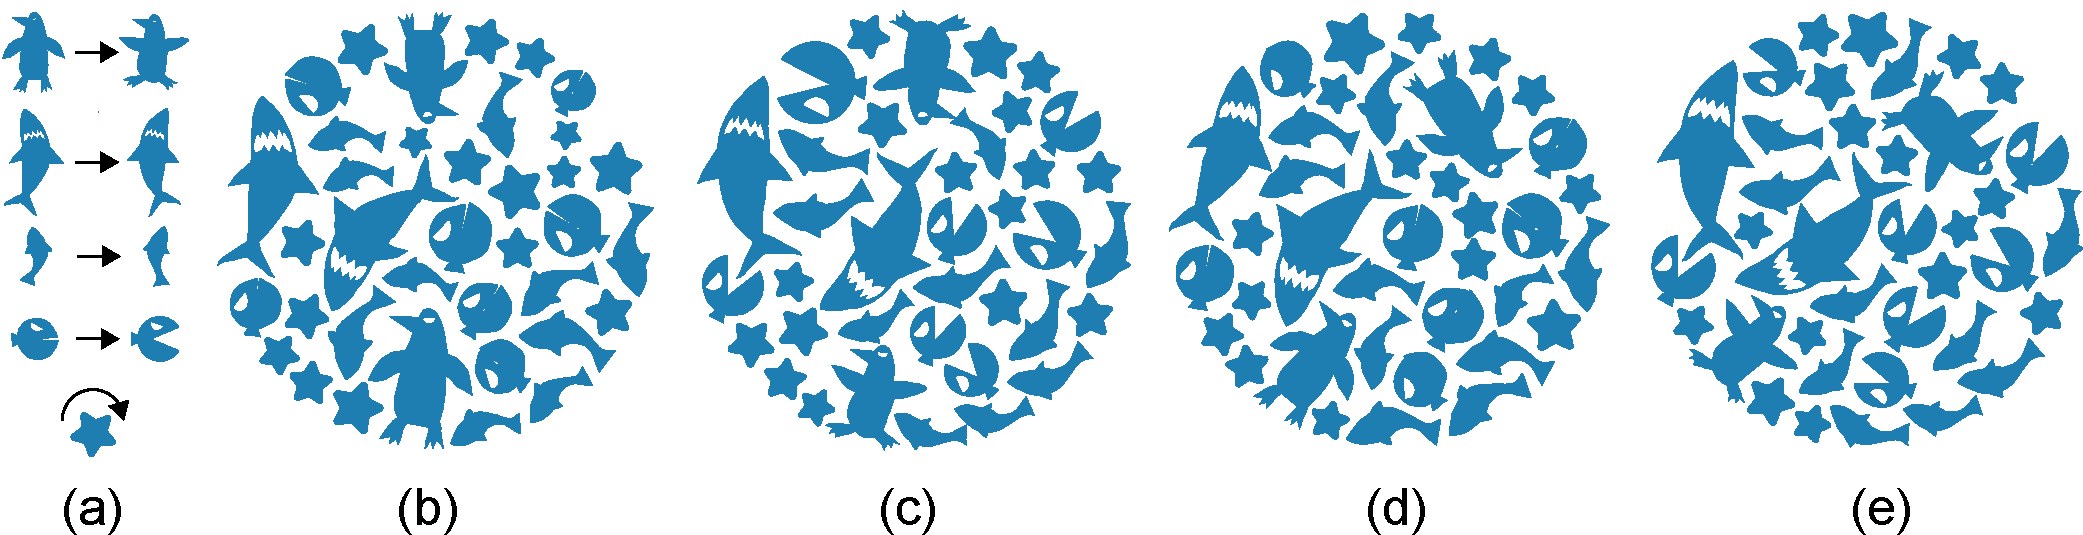
\includegraphics[width=1.0\textwidth]{figures/animationpak/teaser.pdf}
  \caption[An animated packing of aquatic fauna]
  {\label{fig_animationpak_teaser}
  (a) Input animated elements,
  each with its own animation: swimming penguins, swimming sharks and fish,
  Pac-Man fish that open or close their mouths, and rotating stars. 
  (b-e) four selected frames from an animated packing.  
  }
\end{figure*}



%%%%%%%%%%%%%%%%%%%%%%%%%%%%%%%%%%%%%%%%%%%%%%%%%%%%%%%%%%
%%%%%%%%%%%%%%%%%%%%%%%%%%%%%%%%%%%%%%%%%%%%%%%%%%%%%%%%%%
\section{Introduction}
\label{animationpak_introduction}
%%%%%%%%%%%%%%%%%%%%%%%%%%%%%%%%%%%%%%%%%%%%%%%%%%%%%%%%%%
%%%%%%%%%%%%%%%%%%%%%%%%%%%%%%%%%%%%%%%%%%%%%%%%%%%%%%%%%%


AnimationPak is a physics-based packing method for elements with scripted animations.
An element can have an animated deformation, \newtext{such as a slithering snake or a dancing bear}.
It can also have an animated transformation, giving a changing
position, size, and orientation within the container.
Our goal is producing an \textit{animated packing}, with elements
playing out their animations while simultaneously filling the
container shape evenly.  A successful animated packing should balance
among the evenness of the negative space, the preservation of 
element shapes, and the comprehensibility of their scripted animations.

We consider an animated
element to be a geometric extrusion along a time axis, a three-dimensional
object that we call a ``spacetime element''.  We use a three-dimensional physical simulation
similar to RepulsionPak to pack spacetime
elements into a volume created by extruding a static container shape.
The animated packing emerges from this three-dimensional volume by rendering 
cross sections perpendicular to the time axis.

\newtext
{
Animated packings are a largely unexplored style
of motion graphics, presumably because of the difficulty of creating 
an animated packing by hand.  
Finding motivating examples created by artists is difficult.
We only found one shown in Figure~\ref{fig_animationpak_lisa_packing},
which is animated gear-like meshing of copies of Lisa Simpson's spiky head.
The discussion in Section~\ref{animationpak_previous_work} shows there is also very little past research
on animated packings.
}

\begin{figure}[ht]
\centering
\includegraphics[width=1.0\textwidth]{figures/animationpak/lisa_packing.pdf} 
\caption[An animated packing of Lisas from The Simpsons.]
{\label{fig_animationpak_lisa_packing} 
\newtext{Three frames of an animated packing from The Simpsons Season 31, Episode 19 ($\copyright$ FOX), showing
gear-like meshing of oppositely-rotating Lisas.}}
\end{figure}

%%%%%%%%%%%%%%%%%%%%%%%%%%%%%%%%%%%%%%%%%%%%%%%%%%%%%%%%%%
%%%%%%%%%%%%%%%%%%%%%%%%%%%%%%%%%%%%%%%%%%%%%%%%%%%%%%%%%%
\section{Previous Work}
\label{animationpak_previous_work}
%%%%%%%%%%%%%%%%%%%%%%%%%%%%%%%%%%%%%%%%%%%%%%%%%%%%%%%%%%
%%%%%%%%%%%%%%%%%%%%%%%%%%%%%%%%%%%%%%%%%%%%%%%%%%%%%%%%%%

%\mynote{Only discuss papers whose ideas you use or you're comparing with}

\textbf{Packings and Mosaics:} 
Researchers have explored many approaches to creating 2D packings and
simulated mosaics, including using Centroidal Area Voronoi Diagrams (CAVDs) to
position elements~\cite{Hausner2001,Hiller2003,Smith2005}, spectral
approaches to create even negative space~\cite{Dalal2006}, energy
minimization~\cite{Kim2002}, and shape descriptors~\cite{Kwan2016}.
Please refer back to Chapter~\ref{chapter_related_work} 
for a complete list of research in 2D packings.

\textbf{Animated Packings and Tilings:}
Animosaics by Smith et al.~\cite{Smith2005} constructed animations 
in which static elements without scripted
animations follow the motion of an animated container.  Elements are
placed using CAVDs, and advected frame-to-frame using a choice of methods
motivated by Gestalt grouping principles.
As the container's area changes, elements are added and removed as needed,
while attempting to maximize overall temporal coherence.
Dalal et al.~\cite{Dalal2006} showed how the spectral approach they
introduced for 2D packings could be extended 
to pack animated elements in a static container.  Like us, they recast
the problem in terms of three-dimensional spacetime; they compute optimal
element placement using discrete samples over time and orientation.
However, their spacetime elements have fixed
shapes and are made to fit together using only translation and rotation, 
limiting their ability to consume the container's negative space.

Liu and Veksler created animated decorative mosaics from video
input~\cite{Liu2009}.  Their technique combines vision-based
motion segmentation with a packing step similar to Animosaics.
Kang et al.~\cite{Kang2011} extracted edges from video and 
then oriented rectangular tesserae relative to edge directions.

Kaplan~\cite{Kaplan2019} explored animations of simple tilings of
the plane from copies of a single shape.  Elements in a tiling
fit together by construction, and therefore always consume all 
the negative space in the animation.

\textbf{3D Packings:} 
AnimationPak fills a 3D container with 3D elements, 
and is therefore related to other work on constructing freeform 3D
packings, \newtext{although the time axis in the spacetime domain 
behaves differently than the third spatial axis.}
Gal et al.~\cite{Gal2007B} presented a method for constructing 3D
collages reminiscent of portrait paintings by Arcimboldo.  They
filled a 3D container with overlapping 3D elements using a greedy
approach and a partial shape matching algorithm.
Attene~\cite{Attene2015} decomposed a 3D model into parts that pack
tightly into a small build volume, allowing it to 
be 3D printed with less waste material and packed into a smaller box.
Ma et al.~\cite{Ma2018} developed a heuristic method
to create 3D packings that are overlap free.  Other work has 
experimented with example-based packing of 3D volumes~\cite{Ma2011},
or optimized placement based on user interaction~\cite{Hsu2020}.
\newtext{Several approaches have been proposed to extend 2D packing methods to adapt to
the challenges of placing them on the surfaces of 3D 
objects.~\cite{Hu2016,Chen2016,Zehnder2016,Chen2017}.}

\newtext{
\textbf{Animated Textures:}
Ma et al.~\cite{Ma2013} developed Dynamic Element Textures (DET), a method
to synthesize animated textures of a group of identical elements, such as shoals or particles.
For each animated element in a small exemplar, they generate sample points in
spatially and temporally.
To generate a large texture, they copy and distribute the sample points,
which are repositioned to resemble the original point distribution in the exemplar.
Similar to DET, AnimationPak treats an animated element as an object that
resides in a spacetime domain. 
However, as a texture syntesis method,
the goal of DET is to distribute elements, and not fill the negative space.
}

\textbf{Derived Animations:} 
AnimationPak falls into the category of systems that create a derived
animation based on some input animation. This problem, which
requires preserving the visual character of the input, is a 
longstanding one in computer graphics research.
Spacetime constraints~\cite{Witkin1988, Cohen1992} allow an animator
to specify an object's constraints and goals, and then calculates 
the object's trajectory via spacetime optimization.
Motion warping~\cite{Witkin1995} is a method that deforms an existing
motion curve to meet user-specified constraints.
Gleicher~\cite{Gleicher2001} developed a motion path editing method
that allows user to modify the traveling path of a walking character.
Bruderlin and Williams~\cite{Bruderlin1995} used signal processing techniques
to modify motion curves.


Previous work has also investigated geometric deformation of 
animations.
Edmond et al.~\cite{Ho2010} encoded spatial joint relationships 
using tetrahedral meshes, and applied as-rigid-as-possible shape deformation
to the mesh to retarget animation to new characters.
Choi et al.~\cite{Choi2011} developed a method to deform character motion
to allow characters to navigate tight passages.
Masaki~\cite{Oshita2017} developed a motion editing tool that deformed
3D lattice proxies of  a character's joints.
Dalstein et al.~\cite{Dalstein2015} presented a data structure
to animate vector graphics with complex topological changes.
Kim et al.~\cite{Kim2012} explored a packing algorithm
to avoid collisions in a crowd of moving characters.
They defined a motion patch containing temporal trajectories of interacting
characters, and arranged deformed patches to prevent collisions between
characters.


%%%%%%%%%%%%%%%%%%%%%%%%%%%%%%%%%%%%%%%%%%%%%%%%%%%%%%%%%%
%%%%%%%%%%%%%%%%%%%%%%%%%%%%%%%%%%%%%%%%%%%%%%%%%%%%%%%%%%
\section{Animated Elements}
\label{animationpak_animated_element}
%%%%%%%%%%%%%%%%%%%%%%%%%%%%%%%%%%%%%%%%%%%%%%%%%%%%%%%%%%
%%%%%%%%%%%%%%%%%%%%%%%%%%%%%%%%%%%%%%%%%%%%%%%%%%%%%%%%%%

\begin{figure*}
\centering
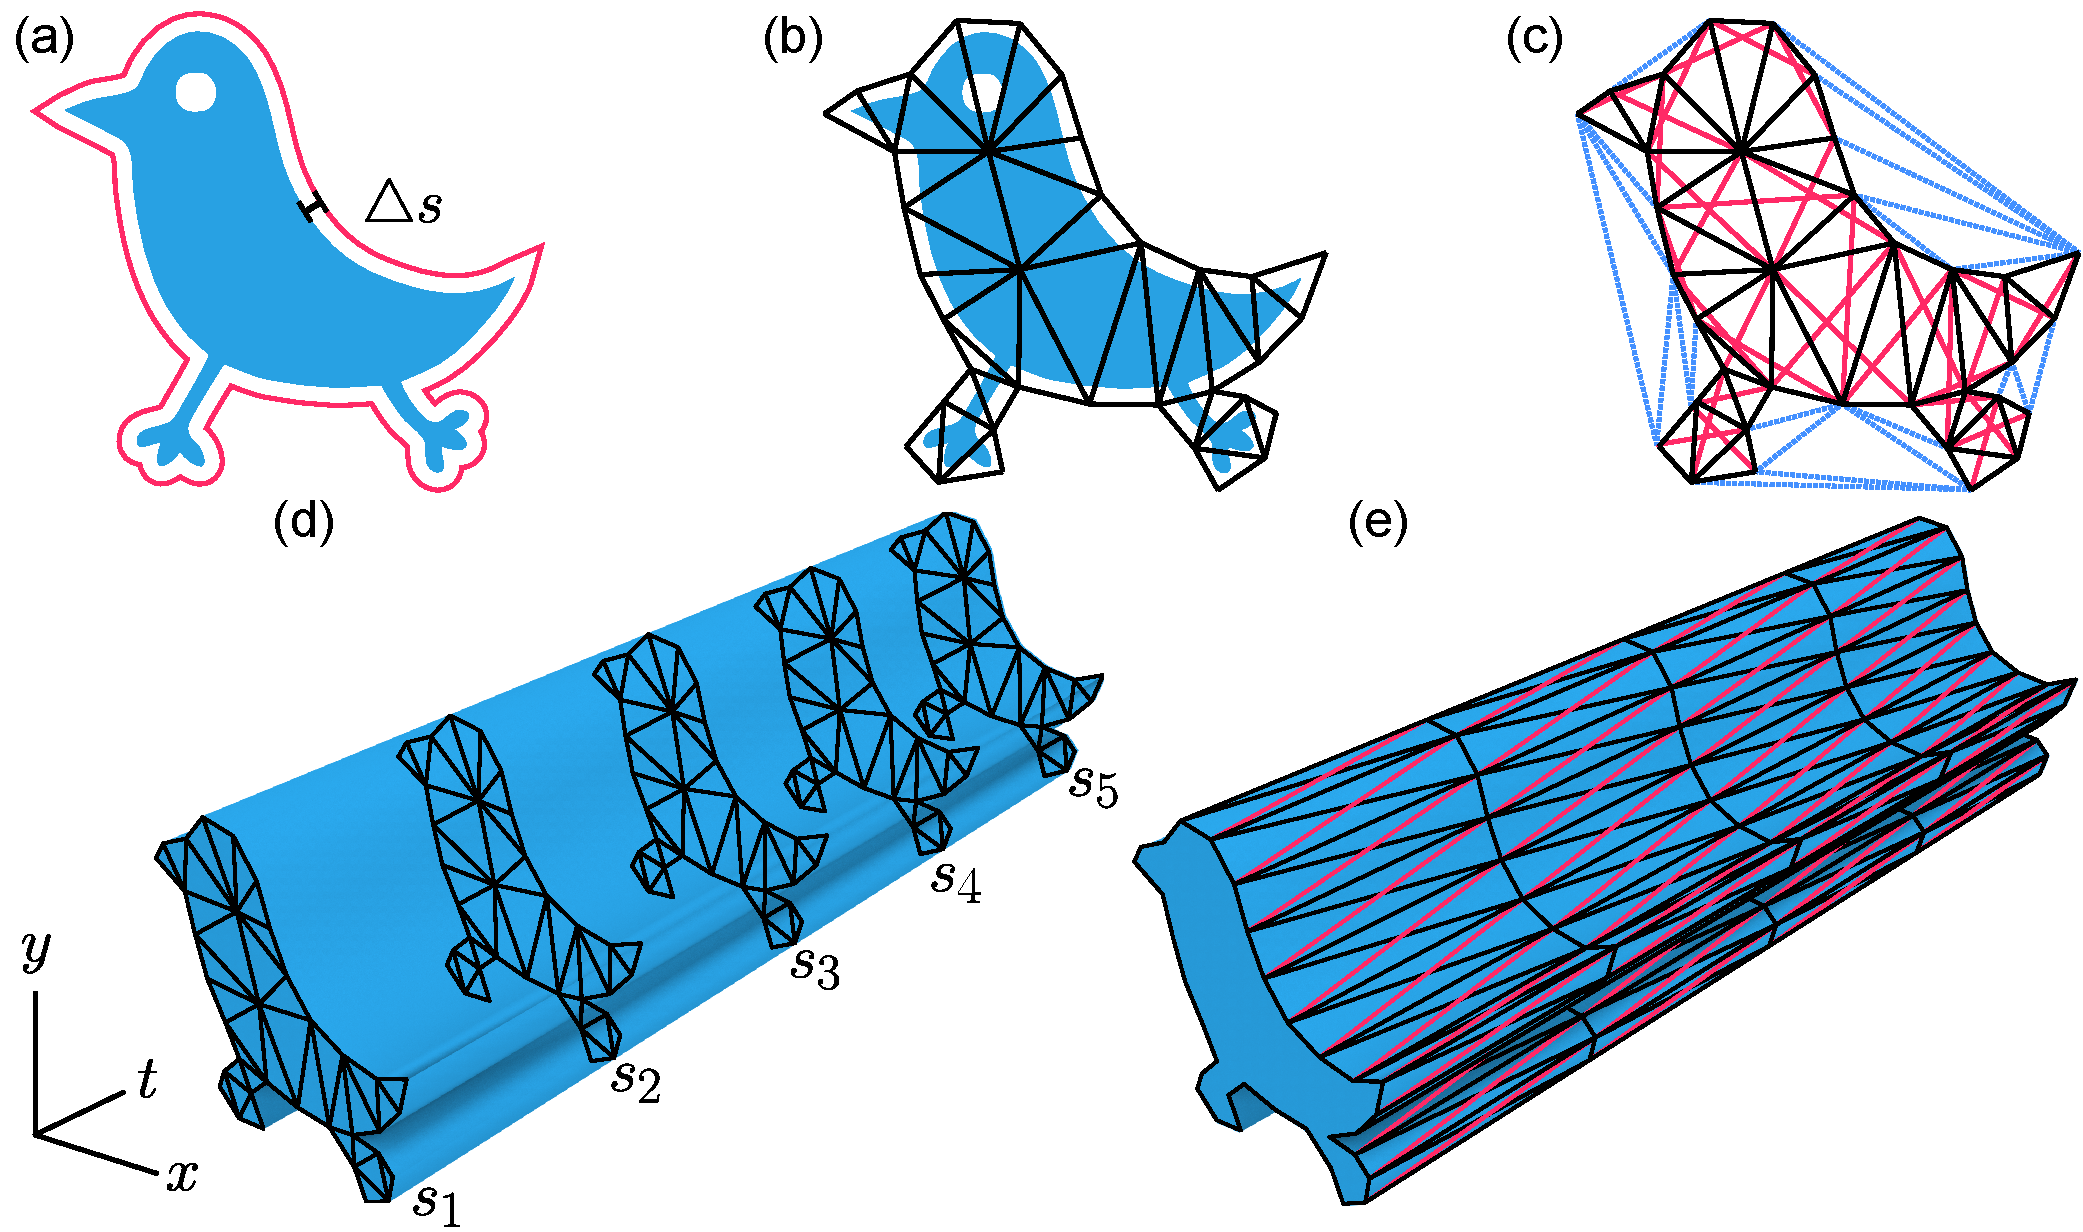
\includegraphics[width=1.0\textwidth]{figures/animationpak/discretization.pdf} 
\caption[The creation of a discretized spacetime element]
{\label{fig_animationpak_discretization} 
The creation of a discretized spacetime element.  
(a) A 2D element shape offset by $\Delta s$.
(b) A single triangle mesh slice.
(c) Shear edges (red) and negative space edges (blue).
(d) A set of five slices placed along the time axis.
(e) The vertices on the boundaries of the slices are joined by 
	time edges.  The black edges in~(e) define a triangle mesh
	called the envelope of the element.
	In practice we use a larger number of slices in~(d) and~(e).
}
\end{figure*}

\begin{figure}
\centering
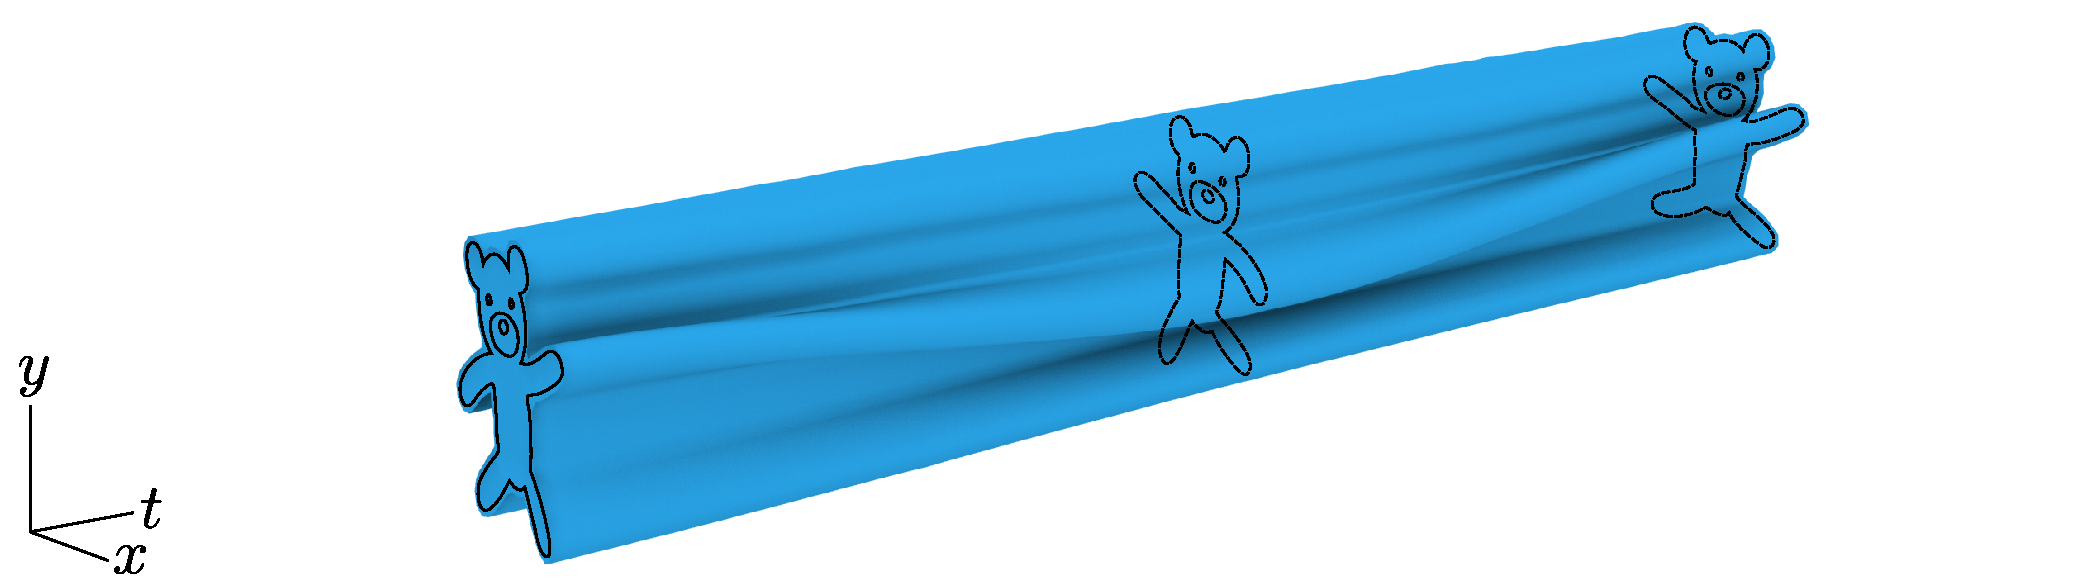
\includegraphics[width=1.0\textwidth]{figures/animationpak/spacetime_element.pdf} 
\caption[A spacetime element with a scripted animation]
{\label{fig_animationpak_spacetime_element} 
A spacetime element with a scripted animation.}
\end{figure}

The input to AnimationPak is a library of animated elements and a
fixed container shape.  AnimationPak currently supports two kinds
of animation: the user can animate the shape of each individual
element and can also give elements trajectories that animate
their position within the container.  This
section explains how we animate the element shapes using
as-rigid-as-possible deformation, and then construct
spacetime-extruded objects that form the basis of our packing
algorithm.  These elements animate ``in place'': they change
shape without translating. The next section describes how these
elements can be given transformation trajectories within the
container. Size and orientation of an element can be animated
either way; they can be specified as an animation of the element's
shape, or they can be part of the transformation trajectory.



%%%%%%%%%%%%%%%%%%%%%%%%%%%%%%%%%%%%%%%%%%%%%%%%%%%%%%%%%%
%%%%%%%%%%%%%%%%%%%%%%%%%%%%%%%%%%%%%%%%%%%%%%%%%%%%%%%%%%
\subsection{Spacetime Extrusion}
\label{animationpak_spacetime_extrusion}
%%%%%%%%%%%%%%%%%%%%%%%%%%%%%%%%%%%%%%%%%%%%%%%%%%%%%%%%%%
%%%%%%%%%%%%%%%%%%%%%%%%%%%%%%%%%%%%%%%%%%%%%%%%%%%%%%%%%%

Each element begins life as a static shape defined using
vector paths.  \newtext{Similar to RepulsionPak}, we construct a discrete
geometric proxy of the element that will interact with other
proxies in a physical simulation.  The construction of this proxy
for a single shape is shown in Figure~\ref{fig_animationpak_discretization}, and
the individual steps are explained in greater detail below.

In order to produce a packing with an even distribution of negative
space, we first offset the shape's paths by a distance $\Delta s$,
leaving the shape surrounded by a channel of negative space
(Figure~\ref{fig_animationpak_discretization}a).  In our system
we scale the shape to fit a unit square and set $\Delta s=0.04$.

\newtext
{
Next, we place evenly-spaced samples around the outer boundary of 
the offset path and construct a Delaunay triangulation of the samples
(Figure~\ref{fig_animationpak_discretization}b). We will
later treat the edges of the triangulation as springs, allowing the
element to deform in response to forces in the simulation.  
We also follow RepulsionPak by adding shear edges to prevent
folding and negative-space edges to avoid self-overlaps during simulation
(Figure~\ref{fig_animationpak_discretization}c).
}

We refer to the augmented triangulation shown in 
Figure~\ref{fig_animationpak_discretization}c as a \textit{slice}.  
The entire spacetime packing process operates on slices.  
However, we will eventually
need to compute deformed copies of the element's original vector paths 
when rendering a final animation (Section~\ref{animationpak_rendering}).
To that end, we re-express all path information relative to the
slice triangulation: every path control point is represented using
barycentric coordinates within one triangle.

To extend the element into the time dimension, 
we now position evenly-spaced copies of the slice along the time axis.
Assuming that the animation will run over the time interval $[0,1]$, 
we choose a number of slices $n_s$ and place slices $\{s_1,\ldots,s_{n_s}\}$,
with slice $s_i$ being placed at time $(i-1)/(n_s-1)$.
Higher temporal resolution will
produce a smoother final animation at the expense of more computation.
In our examples, we set $n_s=100$. 
Figure~\ref{fig_animationpak_discretization}d shows a set of time slices, with
$n_s=5$ for visualization purposes.

To complete the construction of a spacetime element without animation,
we stitch the slices together into a single 3D object.  Let $s_j$ and
$s_{j+1}$ be consecutive slices constructed above.  The outer boundaries
of the element triangulations are congruent polygons offset in the time 
axis.  We stitch the two polygons together using a new set of 
\textit{time edges}: if $AB$ is an edge on the boundary of $s_j$ and
$CD$ is the corresponding edge on the boundary of $s_{j+1}$, then
we add time edges $AC$, $AD$, and $BC$.
During simulation, time edges will transmit forces backwards and forwards in
time, maintaining temporal coherence by smoothing out deformation and 
transformations.
Figure~\ref{fig_animationpak_discretization}e shows time edges for $n_s=5$.


%%%%%%%%%%%%%%%%%%%%%%%%%%%%%%%%%%%%%%%%%%%%%%%%%%%%%%%%%%
%%%%%%%%%%%%%%%%%%%%%%%%%%%%%%%%%%%%%%%%%%%%%%%%%%%%%%%%%%
\subsection{Animation}
\label{animationpak_animation}
%%%%%%%%%%%%%%%%%%%%%%%%%%%%%%%%%%%%%%%%%%%%%%%%%%%%%%%%%%
%%%%%%%%%%%%%%%%%%%%%%%%%%%%%%%%%%%%%%%%%%%%%%%%%%%%%%%%%%

The 3D information constructed above is a parallel extrusion of a 
slice along the time axis, representing a shape with no scripted animation.
We created a simple interactive application for adding animation to
spacetime elements, inspired by as-rigid-as-possible shape
manipulation~\cite{Igarashi2005}.  The artist first designates a subset
of the slices as keyframes.  They can then interactively manipulate
any triangulation vertex of a keyframe slice.  Any vertex that has
been positioned manually has its entire trajectory through the animation
computed using spline interpolation.  Then, at any other slice, the positions
of all other vertices can be interpolated using the as-rigid-as-possible
technique.  The result is a smoothly animated spacetime volume like the one
visualized in Figure~\ref{fig_animationpak_spacetime_element}.

Unlike data-driven packing methods like PAD~\cite{Kwan2016}, methods that
allow distortions do not require a large library of distinct elements
to generate successful packings.  The results in this paper all use
fewer than ten input elements, and some use only one.
The physical simulation induces deformation to enhance 
the compatibility of nearby shapes in the final animation.

%%%%%%%%%%%%%%%%%%%%%%%%%%%%%%%%%%%%%%%%%%%%%%%%%%%%%%%%%%
%%%%%%%%%%%%%%%%%%%%%%%%%%%%%%%%%%%%%%%%%%%%%%%%%%%%%%%%%%
\section{Initial Configuration}
\label{animationpak_initial_configuration}
%%%%%%%%%%%%%%%%%%%%%%%%%%%%%%%%%%%%%%%%%%%%%%%%%%%%%%%%%%
%%%%%%%%%%%%%%%%%%%%%%%%%%%%%%%%%%%%%%%%%%%%%%%%%%%%%%%%%%

\begin{figure}[t]
\centering
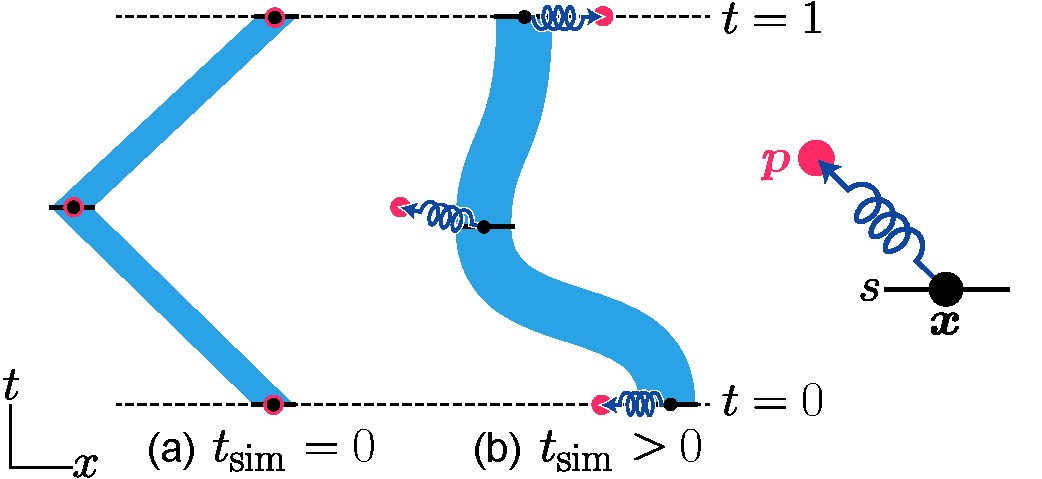
\includegraphics[width=1.0\textwidth]{figures/animationpak/guided_element.pdf} 
\caption[A 2D illustration of a guided element]{
\label{fig_animationpak_guided_element} A 2D illustration of a guided element.
Slices are depicted as black lines and slice vertices as black dots.
A spring connects the centermost vertex $\bm{x}$ of a slice $s$ to a target
point $p$.
(a) The initial shape of a guided element is a polygonal extrusion.
(b) The spacetime element deforms but the springs pull it back towards
the target points.}
\end{figure}

\begin{figure*}[t]
\centering
\includegraphics[width=1.0\textwidth]{figures/animationpak/simulation_process.pdf} 
\caption[AnimationPak simulation process]{
\label{fig_animationpak_simulation_process} The simulation process. 
(a) Initial placement of 
shrunken spacetime elements inside a static 2D disc, extruded into a 
cylindrical spacetime domain.
Guided elements are shown in red and unguided elements in blue.
(b) A physics simulation causes the spacetime elements to bend. They
also grow gradually.
(c) The spacetime elements occupy the container space.
(d) The simulation stops when elements do not have sufficient negative
space in which to grow, or have reached their target sizes.
}
\end{figure*}

We begin the packing process by constructing a 3D spacetime volume for
the container by extruding its static shape in
the time direction.  The container is 
permitted to have internal holes, which are also extruded.  
The resulting volume is scaled to fit a unit cube.
We also shrink each of the spacetime elements, in the spatial dimensions
only, to 5--10\% of its original size.  These shrunken elements are 
thin enough that we can place them in the container without overlaps.


The artist can optionally specify 
trajectories for a subset of the elements, which we call \textit{guided
elements}.  A guided element attempts to pass through a sequence
of fixed target points in the container,
imbuing the animation with a degree
of intention and narrative structure.  To define a guided element,
we designate the triangulation vertex closest to its centroid
to be the anchor point for the element.  The artist then
chooses a set of spacetime target points $\bm{p}_1,\ldots,\bm{p}_n$,
with $\bm{p}_i=(x_i,y_i,t_i)$, that the anchor should pass through
during the animation.
In our interface, the artist uses a slider to choose the time $t_i$ for 
a target point, and clicks in the container to specify the spatial
position $(x_i,y_i)$.
The artist can also optionally specify scale and
orientation at the target points. We require $t_1=0$ and $t_n=1$,
fixing the initial and final positions of the guided element.  
We then linearly interpolate the anchor position
for each slice based on the target points, and translate the slice
so that its anchor lies at the desired position.  The red extrusions
in Figure~\ref{fig_animationpak_simulation_process}a are guided elements.

If the artist wishes to create a looping animation, the $(x_i,y_i)$ position
for target points $\bm{p}_1$ and $\bm{p}_n$ must match up, either
for a single guided element or across elements. In
Figure~\ref{fig_animationpak_simulation_process} the two guided elements form a connected
loop; $(x_1,y_1)$ for each one matches $(x_n,y_n)$ for the other.

In this initial configuration, the guided elements abruptly change
direction at target points.  However, because the slices are connected
by springs, the trajectories will smooth out as the 
simulation runs. Also, the simulation is not constrained to reach
each target position exactly.  Instead, we attach the
anchor to the target using a \textit{target-point spring} that
attempts to draw the element towards it while balancing against
the other physical forces in play (Figure~\ref{fig_animationpak_simulation_process}b).
The strength of these springs determines how closely the element
will follow the trajectory.

We then seed the container with an initial packing of non-guided
spacetime elements.  We generate points within the container at random, 
using blue-noise sampling~\cite{Bridson2007}
to prevent points from being too close together,
and assign a spacetime element to
each seed point, selecting elements randomly from the input library.
Depending upon the desired effect, we either randomize their orientations
or give them preferred orientations.  We reject any candidate seed point
that would cause an unguided element's volume to intersect a guided element's
volume.

Finally we shrink each element, guided and unguided, uniformly in the spatial dimension
towards its centroid.  These shrunken elements are
guaranteed not to intersect one another; as the simulation runs, they
will grow and consume the container's negative space, while avoiding
collisions.
The blue extrusions in Figure~\ref{fig_animationpak_simulation_process}a show an
initial placement of spacetime elements.


%%%%%%%%%%%%%%%%%%%%%%%%%%%%%%%%%%%%%%%%%%%%%%%%%%%%%%%%%%
%%%%%%%%%%%%%%%%%%%%%%%%%%%%%%%%%%%%%%%%%%%%%%%%%%%%%%%%%%
\section{Simulation}
\label{animationpak_simulation}
%%%%%%%%%%%%%%%%%%%%%%%%%%%%%%%%%%%%%%%%%%%%%%%%%%%%%%%%%%
%%%%%%%%%%%%%%%%%%%%%%%%%%%%%%%%%%%%%%%%%%%%%%%%%%%%%%%%%%

%\subsection{Forces}
%\label{animationpak_forces}

\begin{figure} [t]
\centering
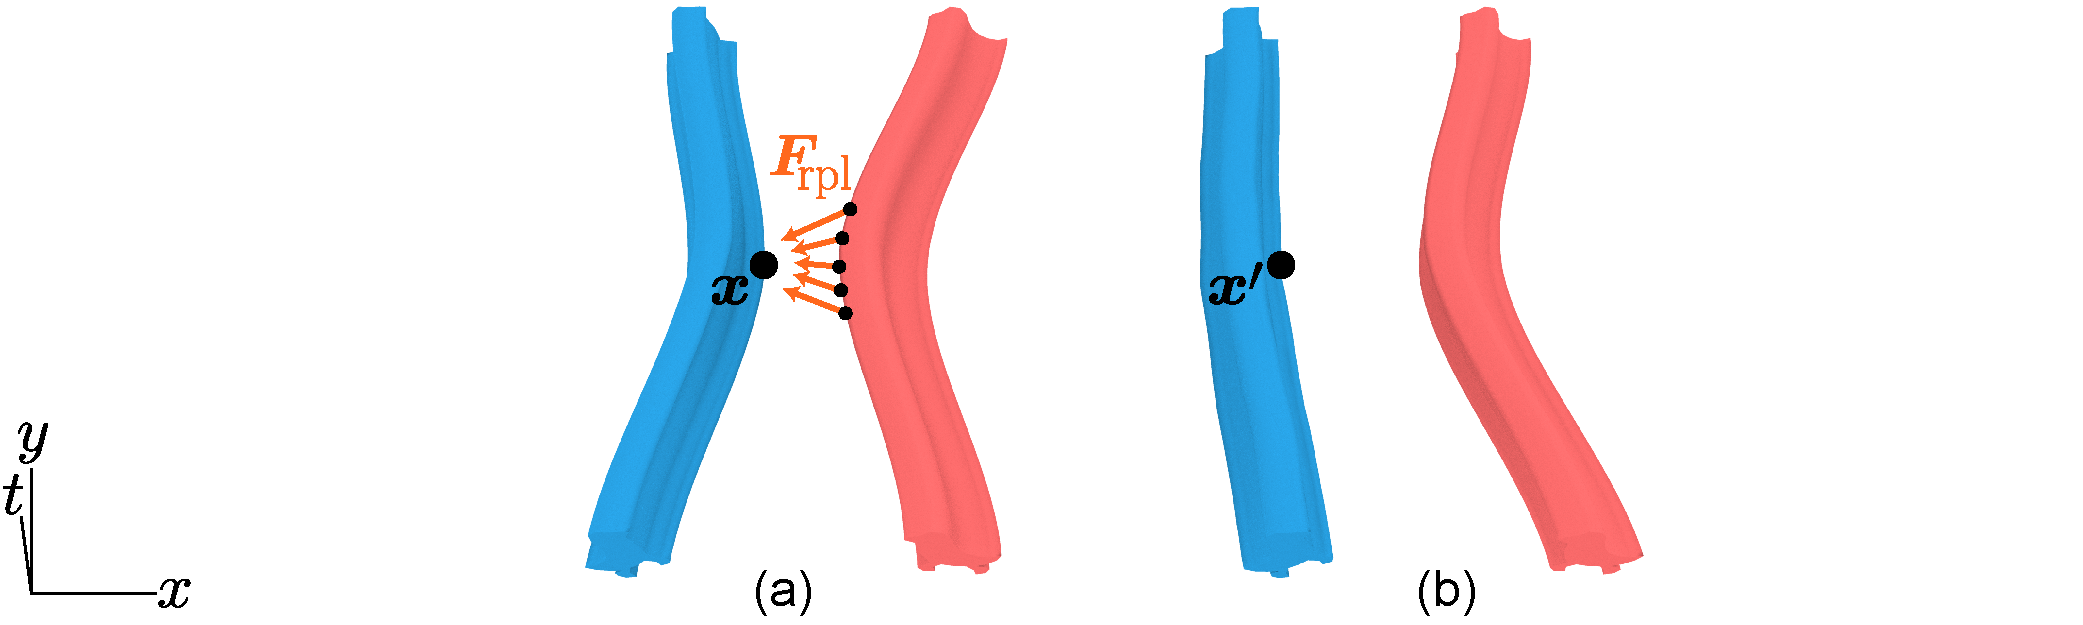
\includegraphics[width=1.0\textwidth]{figures/animationpak/repulsion_force.pdf} 
\caption[Repulsion forces applied to a vertex]
{\label{fig_animationpak_repulsion_force} 
Repulsion forces applied to a vertex $\bm{x}$, 
allowing the element to deform and move away from a neighbouring element.}
\end{figure}

\begin{figure}[t]
\centering
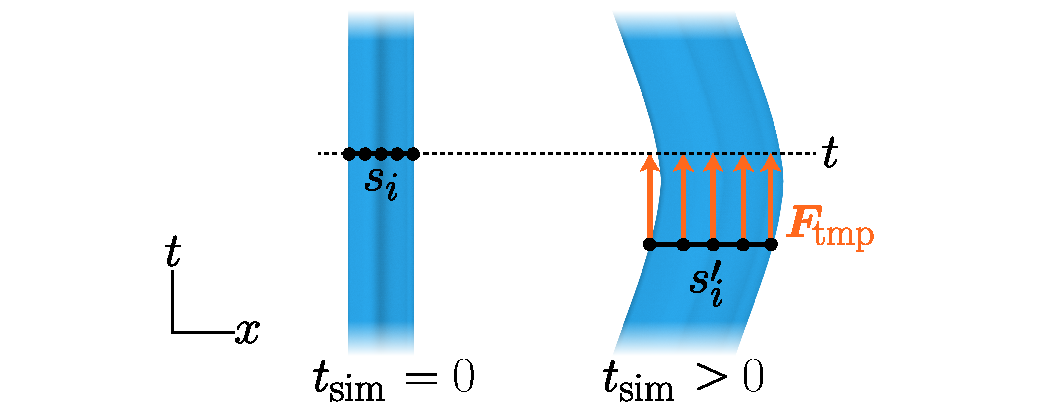
\includegraphics[width=1.0\textwidth]{figures/animationpak/t_force.pdf} 
\caption[An illustration of the temporal force]
{\label{fig_animationpak_t_force} 
An illustration of the temporal force.  The vertices in slice
$s_i$ are drawn back towards time $t$.
}
\end{figure}

\newtext
{
We perform a physics simulation on the spacetime elements and the 
container.  Elements are subject to a number of forces that cause them
to simultaneously grow, deform, and repel each other (Figure~\ref{fig_animationpak_simulation_process}).
In Section~\ref{animationpak_slice_constraints} we introduce some new hard
constraints that must be applied after every time step.
Note that we must distinguish two notions of time in this simulation.  We use
$t$ to refer to the time axis of our spacetime volume, which will become
the time dimension of the final animation, and $t_\mathrm{sim}$ to
refer to the time domain in which the simulation is taking place.
}

\newtext
{
Let $\bm{x} = (x, y, t)$ be a vertex of a slice.
The total force $\simforce{total} $ applied to $\bm{x}$ is
\begin{equation}
\simforce{total}  = \simforce{rpl} + \simforce{edg} + \simforce{bdr} + \simforce{ovr} + \simforce{tor} + \simforce{tmp}
\end{equation}
where $\simforce{rpl}$, $\simforce{edg}$, $\simforce{bdr}$, $\simforce{ovr}$,  $\simforce{tor}$ and $\simforce{tmp}$ are 
the repulsion force, the edge force, the boundary force, the overlap force, the torsional force, and the temporal force.
The these forces are the spacetime analogues of the ones used in RepulsionPak, except the new temporal force.
In this section, we explain the first five forces briefly 
so readers can refer back to Section~\ref{repulsionpak_simulation}
for more details.
}

\newtext
{
\textbf{Repulsion forces} allow elements to push away vertices of 
neighbouring elements, inducing deformations and transformations that lead 
to an even distribution of elements within the container
(Figure~\ref{fig_animationpak_repulsion_force}).
The relative strength of repulsion forces $k_\mathrm{rpl}$ is set to $10$.
Since the simulation operates in the spacetime domain,
vertex $\bm{x}$ accumulates repulsion forces from points at
various time positions.
To locate these points on neighbouring elements that are considered 
nearest, we use a collision grid data structure, described in greater
detail in Section~\ref{animationpak_spatial_queries}.
}

\newtext
{
\textbf{Edge forces}
allow elements to deform in response to repulsion forces.
The edges defined in Section~\ref{animationpak_spacetime_extrusion} are used here as springs.
We have five types of springs, with stiffness constants that can be 
set independently.  In our implementation we set $k_\mathrm{edg}$ 
to $0.01$ for time springs, $0.1$ for negative-space springs,
and 10 for edge springs, shear springs, and target point springs.
}

\newtext
{
\textbf{Overlap forces} resolve a vertex penetrating a
neighboring spacetime element.
Overlaps can occur later in the simulation when negative space is 
limited.  Once we detect a penetration,  
we temporarily disable the repulsion force on vertex $\bm{x}$, and apply
an overlap force $\simforce{ovr}$ to push it out.
The relative strength of overlap forces $k_\mathrm{ovr}$ is set to $5$.
}

\newtext
{
\textbf{Boundary forces} keep vertices inside the container.
If an element vertex $\bm{x}$
is outside the container, the boundary force $\simforce{bdr}$ moves
it towards the closest point
on the container's boundary by an amount proportional to the distance to
the boundary.
The relative strength of boundary forces $k_\mathrm{bdr}$ is set to $5$.
}

\newtext
{
\textbf{Torsional forces} allow an element's slices to be given
preferred orientations, to which they attempt to return.
The relative strength of torsional forces $k_\mathrm{tor}$ is set to $0.1$.
}

\newtext
{
\textbf{Temporal forces} prevent slices from drifting too far
from their original positions along the time axis positions
(Fig.~\ref{fig_animationpak_t_force}), which could cause unexpected accelerations
and decelerations in the final animation.  For every vertex, we compute
the temporal force $\simforce{tmp}$ as
\begin{equation}
\simforce{tmp} = k_\mathrm{tmp} \bm{u}^t(t - t')
\end{equation}
where
\begin{packeddescriptions}
  \item[$k_\mathrm{tmp}$] is the relative strength of 
    $\simforce{tmp}$. We set $k_\mathrm{tmp} = 1$;
  \item[$t$] is the initial time of the slice to which the vertex belongs;
  \item[$t'$] is the current time value of the vertex; and
  \item[$\bm{u}^t = (0,0,1)$].
\end{packeddescriptions}
}

\newtext
{
\textbf{Numerical Integration:}
We use explicit Euler integration to simulate the motions of the mesh vertices under the
forces described above.  Every vertex has a position and a velocity vector; in
every iteration, we update velocities using forces, and update positions using
velocities.  These updates are scaled by a time step 
$\Delta t_\mathrm{sim}$ that we set to $0.01$.
We cap velocities at $10 \Delta t_\mathrm{sim}$ 
to dissipate extra energy from the simulation.
}

%%%%%%%%%%%%%%%%%%%%%%%%%%%%%%%%%%%%%%%%%%%%%%%%%%%%%%%%%%
%%%%%%%%%%%%%%%%%%%%%%%%%%%%%%%%%%%%%%%%%%%%%%%%%%%%%%%%%%
\subsection{Spatial Queries}
\label{animationpak_spatial_queries}
%%%%%%%%%%%%%%%%%%%%%%%%%%%%%%%%%%%%%%%%%%%%%%%%%%%%%%%%%%
%%%%%%%%%%%%%%%%%%%%%%%%%%%%%%%%%%%%%%%%%%%%%%%%%%%%%%%%%%

\begin{figure}
\centering
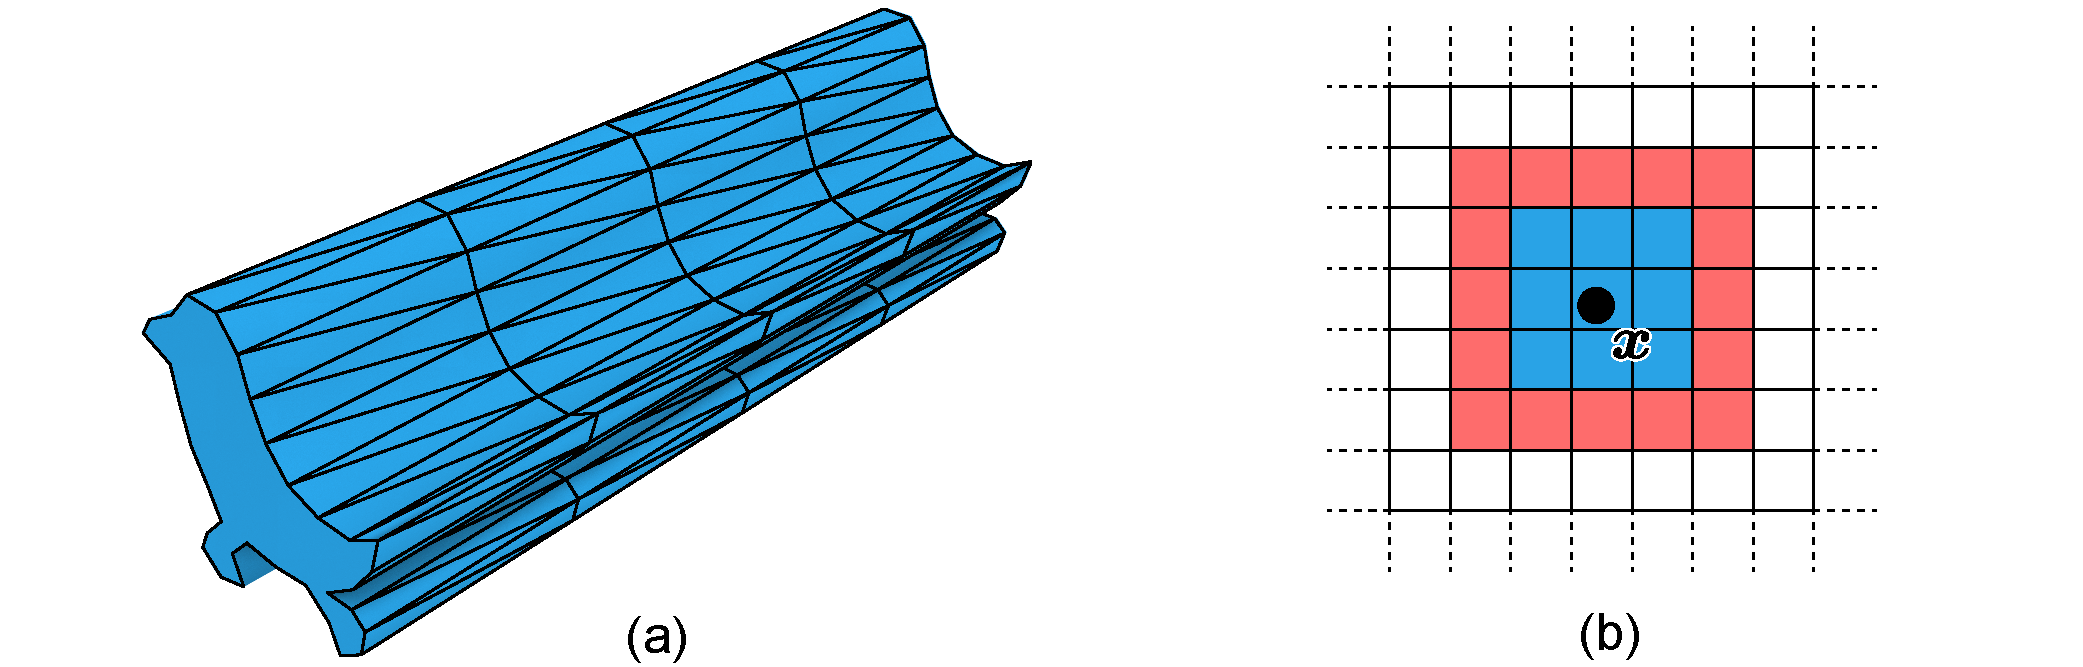
\includegraphics[width=1.0\textwidth]{figures/animationpak/collision_grid.pdf} 
\caption[An envelope and a collision grid]
{\label{fig_animationpak_collision_grid} 
(a) The triangles that connect consecutive slices define the envelope of the
element.  The midpoints of these triangles are stored in a collision grid.
(b) A 2D visualization of the region of collision
grid cells around a query point 
$\bm{x}$ 
in which repulsion and overlap forces will be computed.  In the central blue
region, we check overlaps and compute exact repulsion forces relative to
closest points on triangles of neighbouring elements; in the peripheral
red region we do not compute overlaps, and repulsion forces are approximated
using triangle midpoints only.}
%% \craig{Do we really need this figure?}
\end{figure}

Repulsion and overlap forces rely on being able to find points on
neighbouring elements that are close to a given query vertex.
To find these points, we use each element's
\textit{envelope}, a triangle mesh implied by the construction in
Section~\ref{animationpak_spacetime_extrusion}.  Each triangle of the envelope 
is made from two time edges and one edge of a slice boundary, as
shown in Figure~\ref{fig_animationpak_collision_grid}a.  Given a query vertex 
$\bm{x}$, we need to find nearby envelope triangles that belong to
other elements.

To accelerate this computation, we first find and store the centroids of
every element's envelope triangles in a uniformly subdivided 3D grid that
surrounds the spacetime volume of the animation.  In using this data
structure, we make two simplifying assumptions; first, that because 
envelope triangles are small, their centroids
are adequate for finding triangles near a given query point; and second,
that the repulsion force from a more distant triangle is well approximated
by a force from its centroid.

Given a query vertex $\bm{x}$, we first find all envelope triangle
centroids in nearby grid cells that belong to other elements.  For each 
centroid, we use a method described by Ericson~\cite{Ericson2005} to
find the point on its triangle closest to $\bm{x}$ and
include that point in the list of points in Eq.~(1).  These
nearby triangles will also be used to test for interpenetration of elements.
We then find centroids in more distant grid cells, and add
those centroids directly to the Eq.~(1) list, skipping the closest point computation.
In our system we set the cell size to 0.04, giving a $25\times 25\times 25$
grid around the simulation volume.  A query point's nearby grid cells 
are the 27 cells making up a $3\times 3\times 3$ block around the cell 
containing the point; the more distant cells are the 98 that make up the
outer shell of the $5\times 5\times 5$ block around that 
(Figure~\ref{fig_animationpak_collision_grid}).


%%%%%%%%%%%%%%%%%%%%%%%%%%%%%%%%%%%%%%%%%%%%%%%%%%%%%%%%%%
%%%%%%%%%%%%%%%%%%%%%%%%%%%%%%%%%%%%%%%%%%%%%%%%%%%%%%%%%%
\subsection{Slice Constraints}
\label{animationpak_slice_constraints}
%%%%%%%%%%%%%%%%%%%%%%%%%%%%%%%%%%%%%%%%%%%%%%%%%%%%%%%%%%
%%%%%%%%%%%%%%%%%%%%%%%%%%%%%%%%%%%%%%%%%%%%%%%%%%%%%%%%%%

\begin{figure}[h!]
\centering
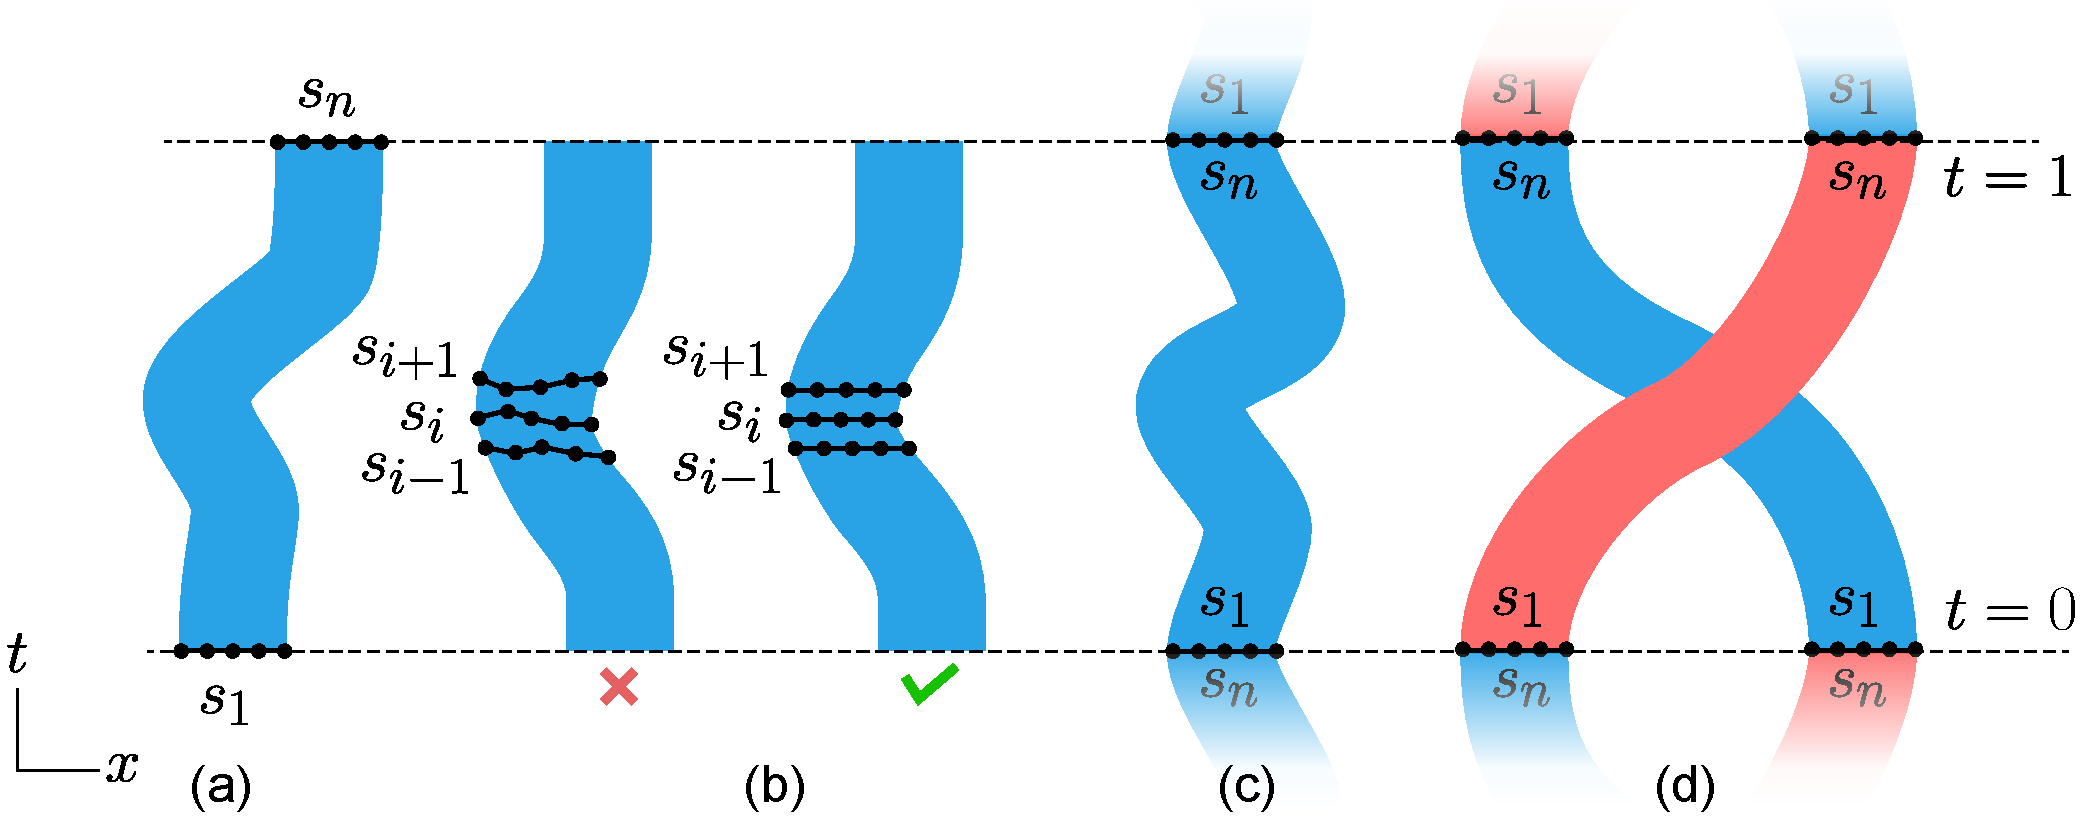
\includegraphics[width=1.0\textwidth]{figures/animationpak/constraints.pdf} 
\caption[Constraints]
{\label{fig_animationpak_constraints} 
a) End-to-end constraint: 
slice $s_1$ and $s_n$, located at 
$t = 0$ and $t = 1$,  should never change their $t$ positions but can change their $x, y$ positions. 
b) Simultaneity constraint: all vertices on the same slice should have the same $t$ position.
c) Loop constraint with a single element: the $x,y$ positions for $s_1$ and $s_n$ must match.
d) Loop constraint with two elements: the $x, y$ position for $s_1$  
for one element matches the $x, y$ position for $s_n$ of the other.
}
\end{figure}



There are three hard geometric constraints on the configuration of slices,
which must be enforced throughout the simulation.  Each of the following
constraints is reapplied after each physical simulation step described above.

\begin{enumerate}
\item \textbf{End-To-End Constraint:}
A spacetime element must be present for the full length of the animation
from $t=0$ to $t=1$.  After every simulation step, every vertex belonging
to an element's first slice has its $t$ value set to $0$, and every vertex
of the last slice has its $t$ value set to $1$
(Figure~\ref{fig_animationpak_constraints}a).

\item \textbf{Simultaneity Constraint:}
During simulation, the vertices of a slice can drift away from each
other in time, which could lead to rendering artifacts in the animation.
After every simulation step, we compute the average $t$ value of all
vertices belonging to each slice other than the first and last slices, and 
snap all the slice's vertices to that $t$ value 
(Figure~\ref{fig_animationpak_constraints}b).

\item \textbf{Loop Constraint:}
AnimationPak optionally supports looping animations.
When looping is enabled, we must ensure that the $t=0$ and $t=1$ planes
of the spacetime container are identical.  
The $t=1$ slice of every element $e_1$ must then 
coincide with the $t=0$ slice of \textit{some} 
element $e_2$.  We can have $e_1=e_2$ 
(Figure~\ref{fig_animationpak_constraints}c), but more general loops are possible in which
the elements arrive at a permutation of their original configuration
(Figure~\ref{fig_animationpak_constraints}d).  We require only that there is a one-to-one
correspondence between the vertices of the $t=1$ slice of $e_1$ and the
$t=0$ slice of $e_2$.  If $\bm{p}_1=(x_1,y_1,1)\in e_1$ and
$\bm{p}_2=(x_2,y_2,0)\in e_2$
are in correspondence, then after every simulation step we
move $\bm{p}_1$ to $(\frac{x_1+x_2}{2},\frac{y_1+y_2}{2},1)$ and
$\bm{p}_2$ to $(\frac{x_1+x_1}{2},\frac{y_2+y_2}{2},0)$.
\end{enumerate}


%%%%%%%%%%%%%%%%%%%%%%%%%%%%%%%%%%%%%%%%%%%%%%%%%%%%%%%%%%
%%%%%%%%%%%%%%%%%%%%%%%%%%%%%%%%%%%%%%%%%%%%%%%%%%%%%%%%%%
\subsection{Element Growth and Stopping Criteria}
\label{animationpak_element_growth_and_stopping_criteria}
%%%%%%%%%%%%%%%%%%%%%%%%%%%%%%%%%%%%%%%%%%%%%%%%%%%%%%%%%%
%%%%%%%%%%%%%%%%%%%%%%%%%%%%%%%%%%%%%%%%%%%%%%%%%%%%%%%%%%

\begin{figure}
\centering
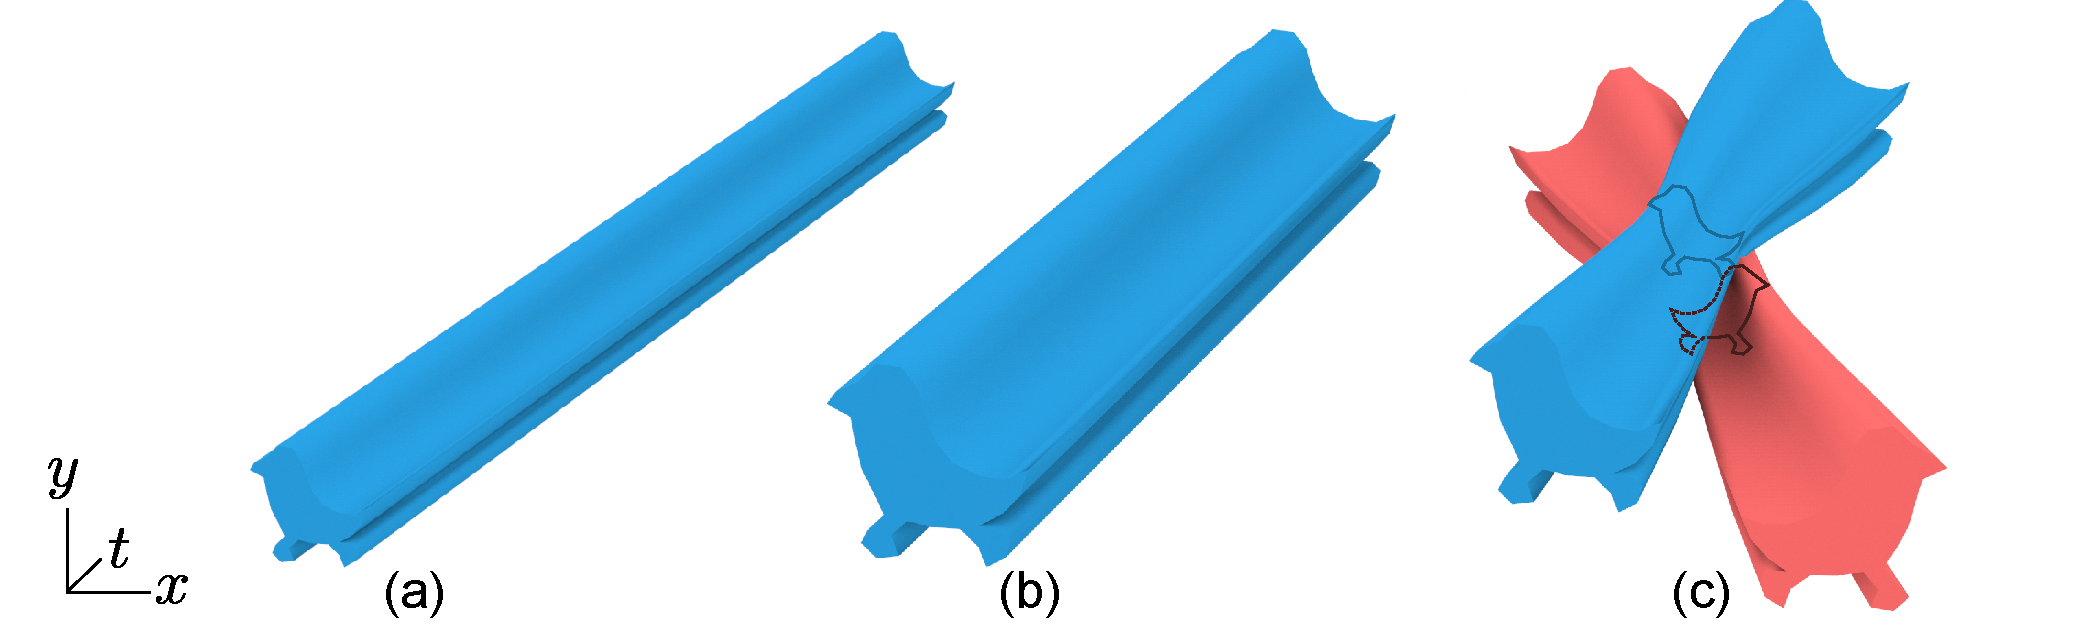
\includegraphics[width=1.0\textwidth]{figures/animationpak/growth.pdf} 
\caption[Element growths]
{\label{fig_animationpak_growth} 
A spacetime element shown (a) shrunken at the beginning of the simulation,
and (b) grown later in the simulation. (c) When two elements overlap
somewhere along their lengths, they are temporarily prohibited from growing
there.
}
\end{figure}

We begin the spacetime packing process with all element slices scaled
down in $x$ and $y$, guaranteeing that elements do not 
overlap.  As the simulation progresses we gradually grow the slices, 
consuming the negative space around them (Figure~\ref{fig_animationpak_growth}a,b).
A perfect packing would fill the spacetime container completely with the elements.
Because each element wraps the underlying animated shape with a narrow channel
of negative space, this would yield an even
distribution of shapes in the resulting animation.
For real-world elements, the goal of minimizing deformation of irregular 
element shapes will lead to imperfect packings with additional pockets
of negative space.


\textbf{Element Growth:}
We induce elements to grow spatially by gradually increasing the rest 
lengths of their springs.
The initial rest length of each spring is determined by the vertex positions in
the shrunken version of the spacetime element constructed in 
Section~\ref{animationpak_initial_configuration}.
We allow an element's slices to grow independently of each other, which
complicates the calculation of new rest lengths for time springs.
Therefore, we create a duplicate of every shrunken spacetime element
in the container, with a straight extrusion
for unguided elements, and a polygonal extrusion for guided elements.
This duplicate is not part of the simulation; it serves as a reference.
Every element slice maintains a current scaling factor $g$.
When we wish to grow the slice, we increase its $g$ value.
We can compute new rest lengths for all springs by scaling every slice
of the reference element by a factor of $g$ relative to the
slice's centroid, and measuring distances between the scaled vertex
positions.  \newtext{These new rest lengths are then used as the $\ell$ values
in Equation~\ref{eq_edge_force} to calculate edge forces.}

Every element slice has its $g$ value initialized to $1$.  After every
simulation step, if none of the slice's vertices were found to 
overlap other elements we increase that slice's $g$ by 
$0.001 \Delta t_\mathrm{sim}$, where $\Delta t_\mathrm{sim}$ is the 
simulation time step.  If any overlaps are found, then that slice's
growth is instead paused to allow overlap and repulsion forces to give it more
room to grow in later iterations.  
This approach can cause elements to fluctuate in size during the course
of an animation, as slices compete for shifting negative space 
(Figure~\ref{fig_animationpak_growth}).

\textbf{Stopping Criteria:} We halt the simulation when the space between
neighbouring elements drops below a threshold.  When calculating 
repulsion forces, we find the distance from every slice vertex
to the closest point in a neighbouring element.  The minimum of these
distances over all vertices in an element slice determines that slice's
closest distance to neighbouring elements.  We halt the simulation
when the maximum per-slice distance falls below 0.006 (relative to a normalized
container size of 1).  That is, we stop when every slice is touching
(or nearly touching) at least one other element.

In some cases it can be useful to stop early based on cumulative element
growth.  In that case, we set a separate threshold for the slice scaling
factors $g$ described above, and stop when the $g$ values of all
slices exceed that threshold.


%%%%%%%%%%%%%%%%%%%%%%%%%%%%%%%%%%%%%%%%%%%%%%%%%%%%%%%%%%
%%%%%%%%%%%%%%%%%%%%%%%%%%%%%%%%%%%%%%%%%%%%%%%%%%%%%%%%%%
\section{Rendering}
\label{animationpak_rendering}
%%%%%%%%%%%%%%%%%%%%%%%%%%%%%%%%%%%%%%%%%%%%%%%%%%%%%%%%%%
%%%%%%%%%%%%%%%%%%%%%%%%%%%%%%%%%%%%%%%%%%%%%%%%%%%%%%%%%%

\begin{figure*}
\centering
\includegraphics[width=1.0\textwidth]{figures/animationpak/rendering.pdf} 
\caption[An illustration of rendering spacetime elements]
{\label{fig_animationpak_render} 
\newtext{
An illustration of rendering spacetime elements to generate 2D frames by cutting them
at evenly spaced time values from $t=0$ to $t=1$.
}
}
\end{figure*}

The result of the simulation described previously is a packing of spacetime 
elements within a spacetime container.  We can render an
animation frame-by-frame by cutting through this volume at 
evenly spaced $t$ values from $t=0$ to $t=1$.  For our results, we
typically render 500-frame animations.


During simulation, a given spacetime element's slices may drift from their
original creation times.  However, time springs keep the sequence
monotonic, and the simultaneity constraint ensures that every slice
is fixed to one $t$ value.  To render this element at an arbitrary
frame time $t_f\in[0,1]$, we find the two consecutive slices whose
time values
bound the interval containing $t_f$ and linearly interpolate the vertex
positions of the triangulations at those two slices to obtain a new
triangulation at $t_f$.  We can then compute a deformed copy of the
original element paths by ``replaying'' the barycentric coordinates 
computed in Section~\ref{animationpak_spacetime_extrusion} relative to the displaced
triangulation vertices.  We repeat this process for every spacetime element
to obtain a rendering of the frame at $t_f$.

This interpolation process can occasionally lead to small artifacts in 
the animation.  A rendered frame can fall between
the discretely sampled slices for two elements at an intermediate time
where physical forces were not computed explicitly.  It is therefore
possible for neighbouring elements to overlap briefly during such intervals.


%%%%%%%%%%%%%%%%%%%%%%%%%%%%%%%%%%%%%%%%%%%%%%%%%%%%%%%%%%
%%%%%%%%%%%%%%%%%%%%%%%%%%%%%%%%%%%%%%%%%%%%%%%%%%%%%%%%%%
\section{Implementation and Results}
\label{animationpak_implementation_and_results}
%%%%%%%%%%%%%%%%%%%%%%%%%%%%%%%%%%%%%%%%%%%%%%%%%%%%%%%%%%
%%%%%%%%%%%%%%%%%%%%%%%%%%%%%%%%%%%%%%%%%%%%%%%%%%%%%%%%%%


The core AnimationPak algorithm consists of a C++ program that reads 
in text files describing the spacetime elements and the container, 
and outputs raster images of animation frames.

Large parts of AnimationPak can benefit from parallelism.  In
our implementation we update the cells of the collision grid
(Section~\ref{animationpak_spatial_queries}) in parallel by distributing them
across a pool of threads.  When the updated collision grid is ready,
we distribute the spacetime elements over threads.  We calculate
forces, perform numerical integration, and apply the end-to-end and
simultaneity constraints for each element in parallel.  We must
process any loop constraints afterwards, as they can affect vertices in
two separate elements.

We created the results in this paper using a Windows PC with a 
3.60GHz Intel i7-4790 processor and 16 GB of RAM.  We used a pool
of eight threads, corresponding to the number of logical CPU cores.
Table~\ref{table_packing_statistics} shows statistics for our results.
Each packing has tens of thousands of vertices and hundreds of thousands
of springs, and requires about an hour to complete.
We enable the loop constraint in all results.  \newtext{This chapter shows selected frames from the
results; see supplemental videos for full animations\footnote{\url{https://cs.uwaterloo.ca/~radhitya/animationpak/videos.zip}}.}

%\begin{comment}
\begin{table}[t!]
\centering 
\caption[Data and statistics for the AnimationPak results]
{
   Data and statistics for the AnimationPak results.  The table shows the
   number of elements,
   the number of vertices, 
   the number of springs, 
    the number of envelope triangles, and 
   the running time of the simulation in hours, minutes, and seconds.
   }
\label{table_packing_statistics}
\definecolor{lg}{rgb}{0.73,0.867,0.98}
\begin{tabular}{|c|c|c|c|c|c|}
\hline
  \cellcolor{lg}Packing &
  \cellcolor{lg}Elements &
  \cellcolor{lg}Vertices & 
  \cellcolor{lg}Springs &
  \cellcolor{lg}Triangles &
  \cellcolor{lg}Time \\ \hline
\makecell{Aquatic fauna  \\ (Figure~\ref{fig_animationpak_teaser})}  
& 37         & 97,800             & 623,634            & 106,000    & 01:06:35        
\\ \hline
\makecell{Snake and birb     \\ (Figure~\ref{fig_animationpak_chasing_bird})}  
& 37         & 58,700             & 370,571            & 58,700   & 01:01:32        
\\ \hline
\makecell{Penguin to giraffe \\ (Figure~\ref{fig_animationpak_penguin_giraffe})}  
& 33         & 124,300            & 824,164            & 143,000    & 01:19:50        
\\ \hline
\makecell{\newtext{Star birds} \\ (Figure~\ref{fig_bib_entering_star})}  
& 32         & 63,700            & 389,373            & 70,100    & 00:19:24        
\\ \hline
\makecell{Lion               \\ (Figure~\ref{fig_animationpak_lion}b)}  
& 16         & 39,400             & 236,086            & 41,800   & 00:41:56        
\\ \hline
\makecell{Animals            \\ (Figure~\ref{fig_animationpak_repulsionpak_vs_animationpak}b)}  
& 34         & 69,600             & 444,337            & 69,800   & 01:00:19        
\\ \hline
\makecell{Heart stars         \\ (Figure~\ref{fig_animationpak_star_comparison}c)}  
& 26         & 85,200             & 598,218            & 85,800   & 00:23:08        
\\ \hline
\end{tabular}
\end{table}



Figure~\ref{fig_animationpak_teaser} is an animation of aquatic fauna featuring two
penguins as guided elements.  During one loop the penguins move clockwise
around the container, swapping positions at the top and the bottom.
Each ends at the other's starting point, demonstrating a loop constraint
between distinct elements.  All elements are animated, as shown in 
Figure~\ref{fig_animationpak_teaser}a.  Note the coupling between the Pac-Man fish's
mouth and the shark's tail on the left side of the second and fourth frames.

A snake chases a bird around an annular container in 
Figure~\ref{fig_animationpak_chasing_bird}, demonstrating a container with a hole
and giving a simple example of the narrative potential of animated
packings.  Figure~\ref{fig_animationpak_penguin_giraffe} animates the giraffe-to-penguin
illusion shown as a static packing in RepulsionPak.  This example
uses torsional forces to control slice orientations.

\newtext{
Figure~\ref{fig_bib_entering_star} shows an loose bird enters and leaves a packing of smaller birds.
This is an example of the benefit of our growth approach.
As the bigger bird is inside the container, available space is more limited,
causing smaller birds to stop some of their slice growths.
In the resulted 2D animation, the non-uniform slice growths create the shrinking effect on 2D elements,
causing them to give up their space to accommodate another element.
}

Figure~\ref{fig_animationpak_lion}a is a static packing of a lion created by an artist and
used as an example in FLOWPAK (Chapter~\ref{chapter_flowpak}).  In Figure~\ref{fig_animationpak_lion}b,
we reproduce it with animated elements for the mane.
The orientations of elements follow a vector field inside
the container, and are maintained during the animation by 
torsional forces.
We simulate only half of the packing and reflect it to create the other half.
The facial features were added manually in a post-processing step.

Figure~\ref{fig_animationpak_repulsionpak_vs_animationpak} compares
a static 2D packing created by RepulsionPak with a frame
from an animated packing created by AnimationPak.
The extra negative space in AnimationPak comes partly from the trade-off
between temporal coherence and tight packing, and partly from the lack
of secondary elements, which were used in a second pass in RepulsionPak 
to fill pockets of negative space.


Figure~\ref{fig_animationpak_star_comparison} offers a direct comparison between
packings computed using Centroidal Area Voronoi Diagrams
(CAVD)~\cite{Smith2005}, the spectral approach~\cite{Dalal2006}, and AnimationPak.
These packings use stars that rotate and pulsate.
For each method we show the initial frame ($t=0$) and the halfway point
($t=0.5$).  The CAVD approach produces a satisfactory---albeit
loosely coupled---packing for the first frame, but because the 
algorithm was not intended to work on animated elements, 
the evenness of the packing quickly degrades in later frames.
The spectral approach is much better
than CAVD, but their animated elements still have fixed spacetime shapes
and can only translate and rotate to improve their fit. 
Repulsion forces and deformation allow AnimationPak to achieve a tighter packing
that persists across the animation, including gear-like meshing of
oppositely-rotating stars.




Figure~\ref{fig_animationpak_teaser_weak_t_springs} emphasizes the trade-off between
temporal coherence and evenness of negative space by creating two animations
with different time springs stiffness.  In (a), the time springs
are 100 times stronger than in (b).  The resulting packing has larger
pockets of negative space, but the accompanying video shows that the
animation is smoother.  The packing in (b) is tighter, but the elements
must move frantically to maintain that tightness.


Figure~\ref{fig_animationpak_blender} is a failed attempt to animate a ``blender''.
The packing has a beam that rotates clockwise
and a number of small unguided circles.  
In a standard physics simulation we might expect the beam to push the 
circles around the container, giving each one a helical spacetime 
trajectory.
Instead, as elements grow, repulsion forces cause circles to explore the 
container boundary, where they discover the lower-energy solution of 
slipping past the edge of the beam as it sweeps past.
If we extend the beam to the full diameter of the container,
consecutive slices simply teleport across the beam, hiding the moment of
overlap in the brief time interval where physical forces were not computed.
AnimationPak is not directly comparable to a
3D physics simulation; it is better suited to improving the
packing quality of an animation that has already been blocked out at a 
high level.


%%%%%%%%%%%%%%%%%%%%%%%%%%%%%%%%%%%%%%%%%%%%%%%%%%%%%%%%%%
%%%%%%%%%%%%%%%%%%%%%%%%%%%%%%%%%%%%%%%%%%%%%%%%%%%%%%%%%%
\section{Conclusions}
\label{animationpak_conclusions}
%%%%%%%%%%%%%%%%%%%%%%%%%%%%%%%%%%%%%%%%%%%%%%%%%%%%%%%%%%
%%%%%%%%%%%%%%%%%%%%%%%%%%%%%%%%%%%%%%%%%%%%%%%%%%%%%%%%%%

We introduced AnimationPak, a system for 
generating animated packings by filling a static container with animated
elements.  Every animated 2D element is represented by an extruded 
spacetime tube.
We discretize elements into triangle mesh slices connected by time edges,
and deform element shapes and animations using a spacetime physical
simulation.  The result is a temporally coherent 2D animation of elements
that attempt both to perform their scripted motions and consume the negative
space of the container.
We show a variety of results where
2D elements move around inside the container.




\begin{figure*}
\centering
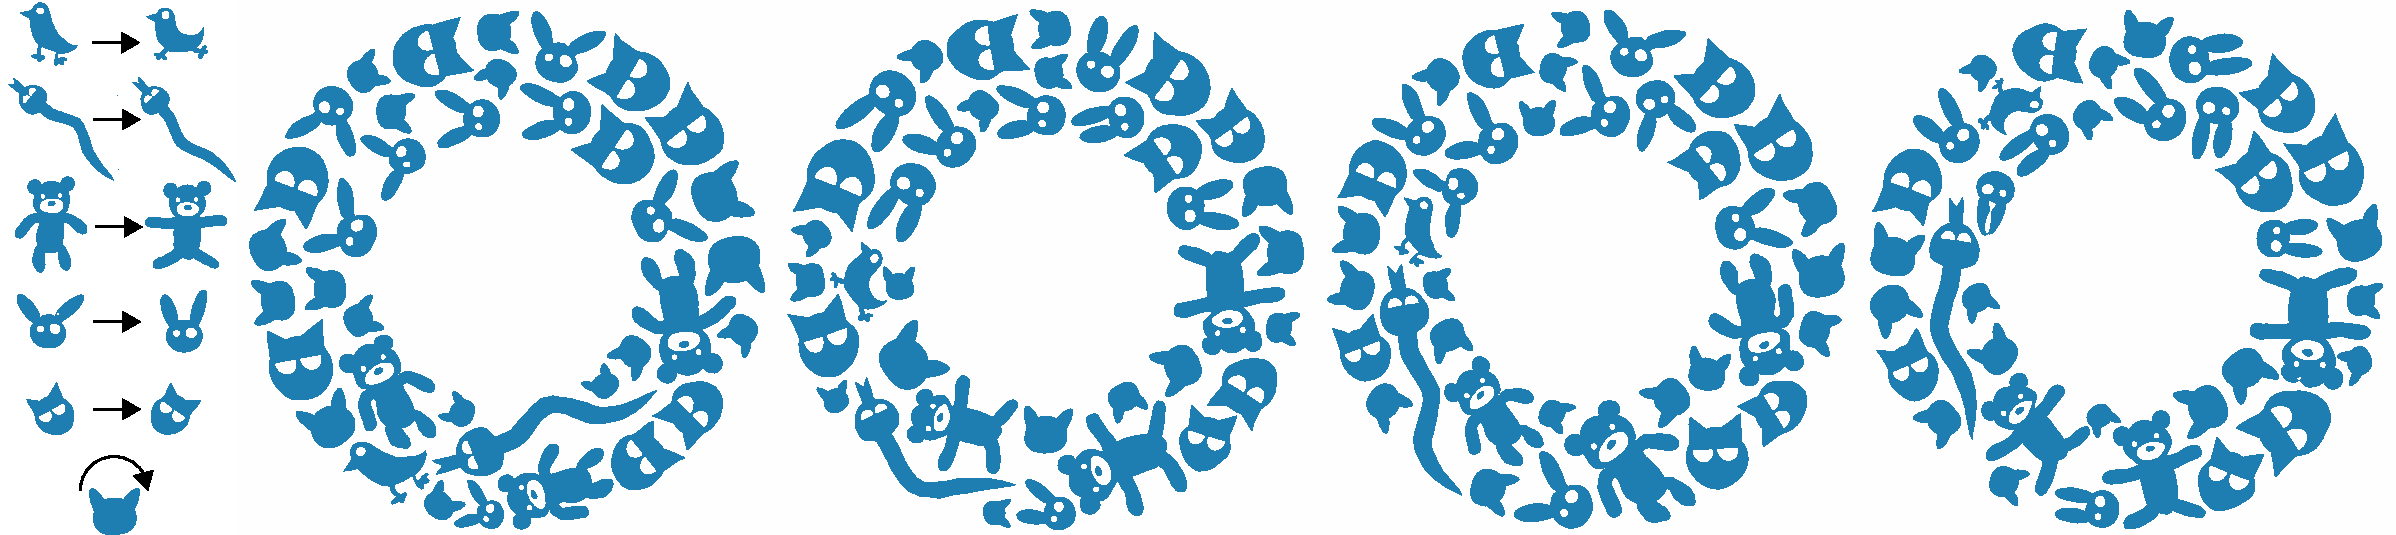
\includegraphics[width=1.0\textwidth]{figures/animationpak/chasing_bird.pdf} 
\caption[An animated packing of a snake chases a bird]
{\label{fig_animationpak_chasing_bird} 
A snake chasing a bird through a packing of animals.  The snake and bird 
	are both guided elements that move clockwise around the annular 
	container.}
\end{figure*}

\begin{figure*}
\centering
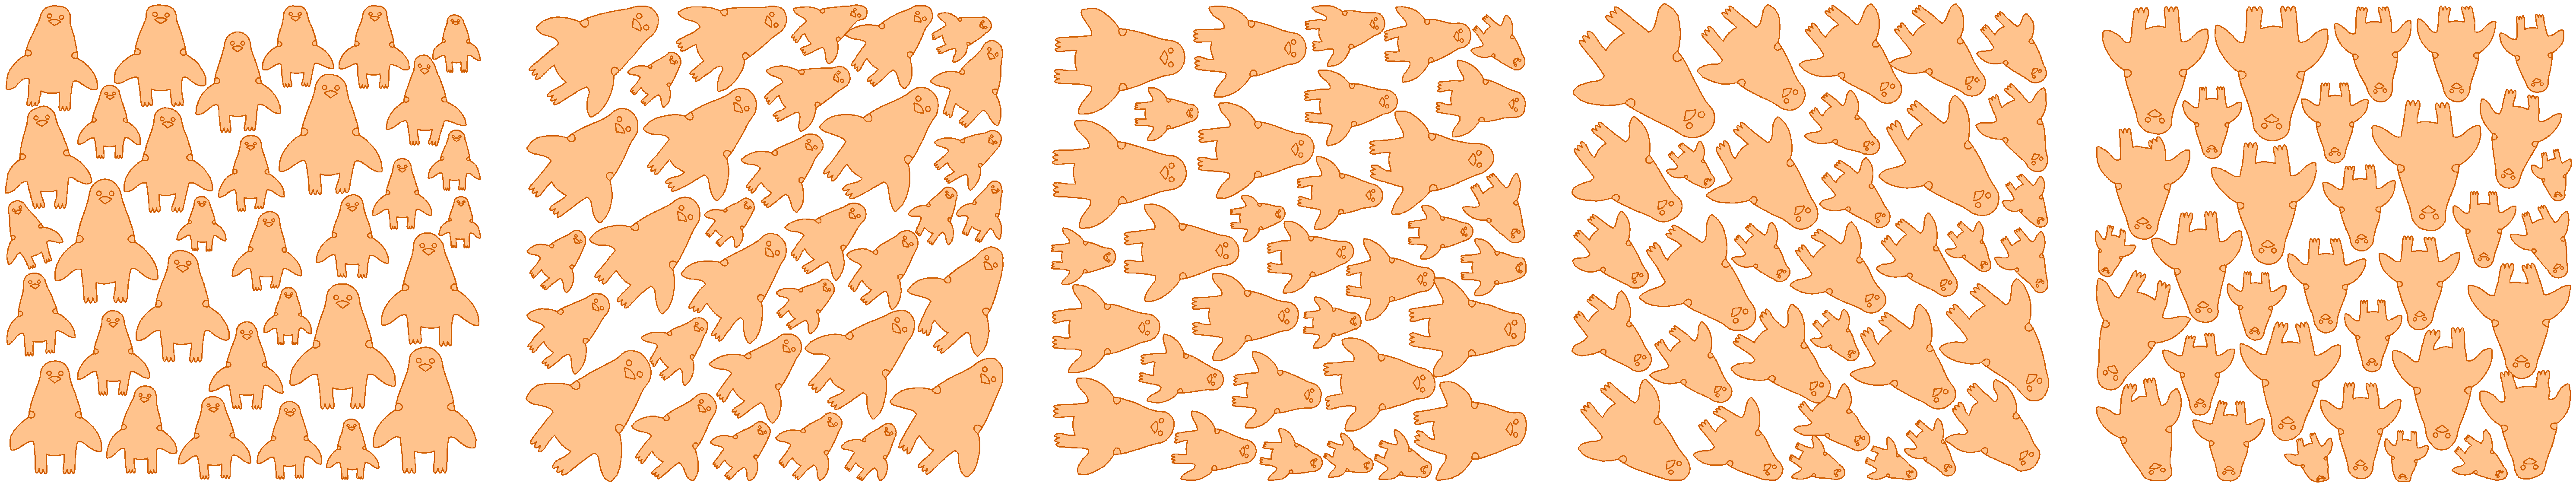
\includegraphics[width=1.0\textwidth]{figures/animationpak/penguin_giraffe.pdf} 
\caption[An animated packing of the penguins-to-giraffes illusion]
{\label{fig_animationpak_penguin_giraffe} 
Penguins turning into giraffes.  The penguins animate by rotating in place.
Torsional forces are used to preserve element orientations.
Frames are taken at $t=0$, $t=0.125$, $t=0.25$, $t=0.375$, and $t=0.5$. 
}
\end{figure*}


\begin{figure*}
\centering
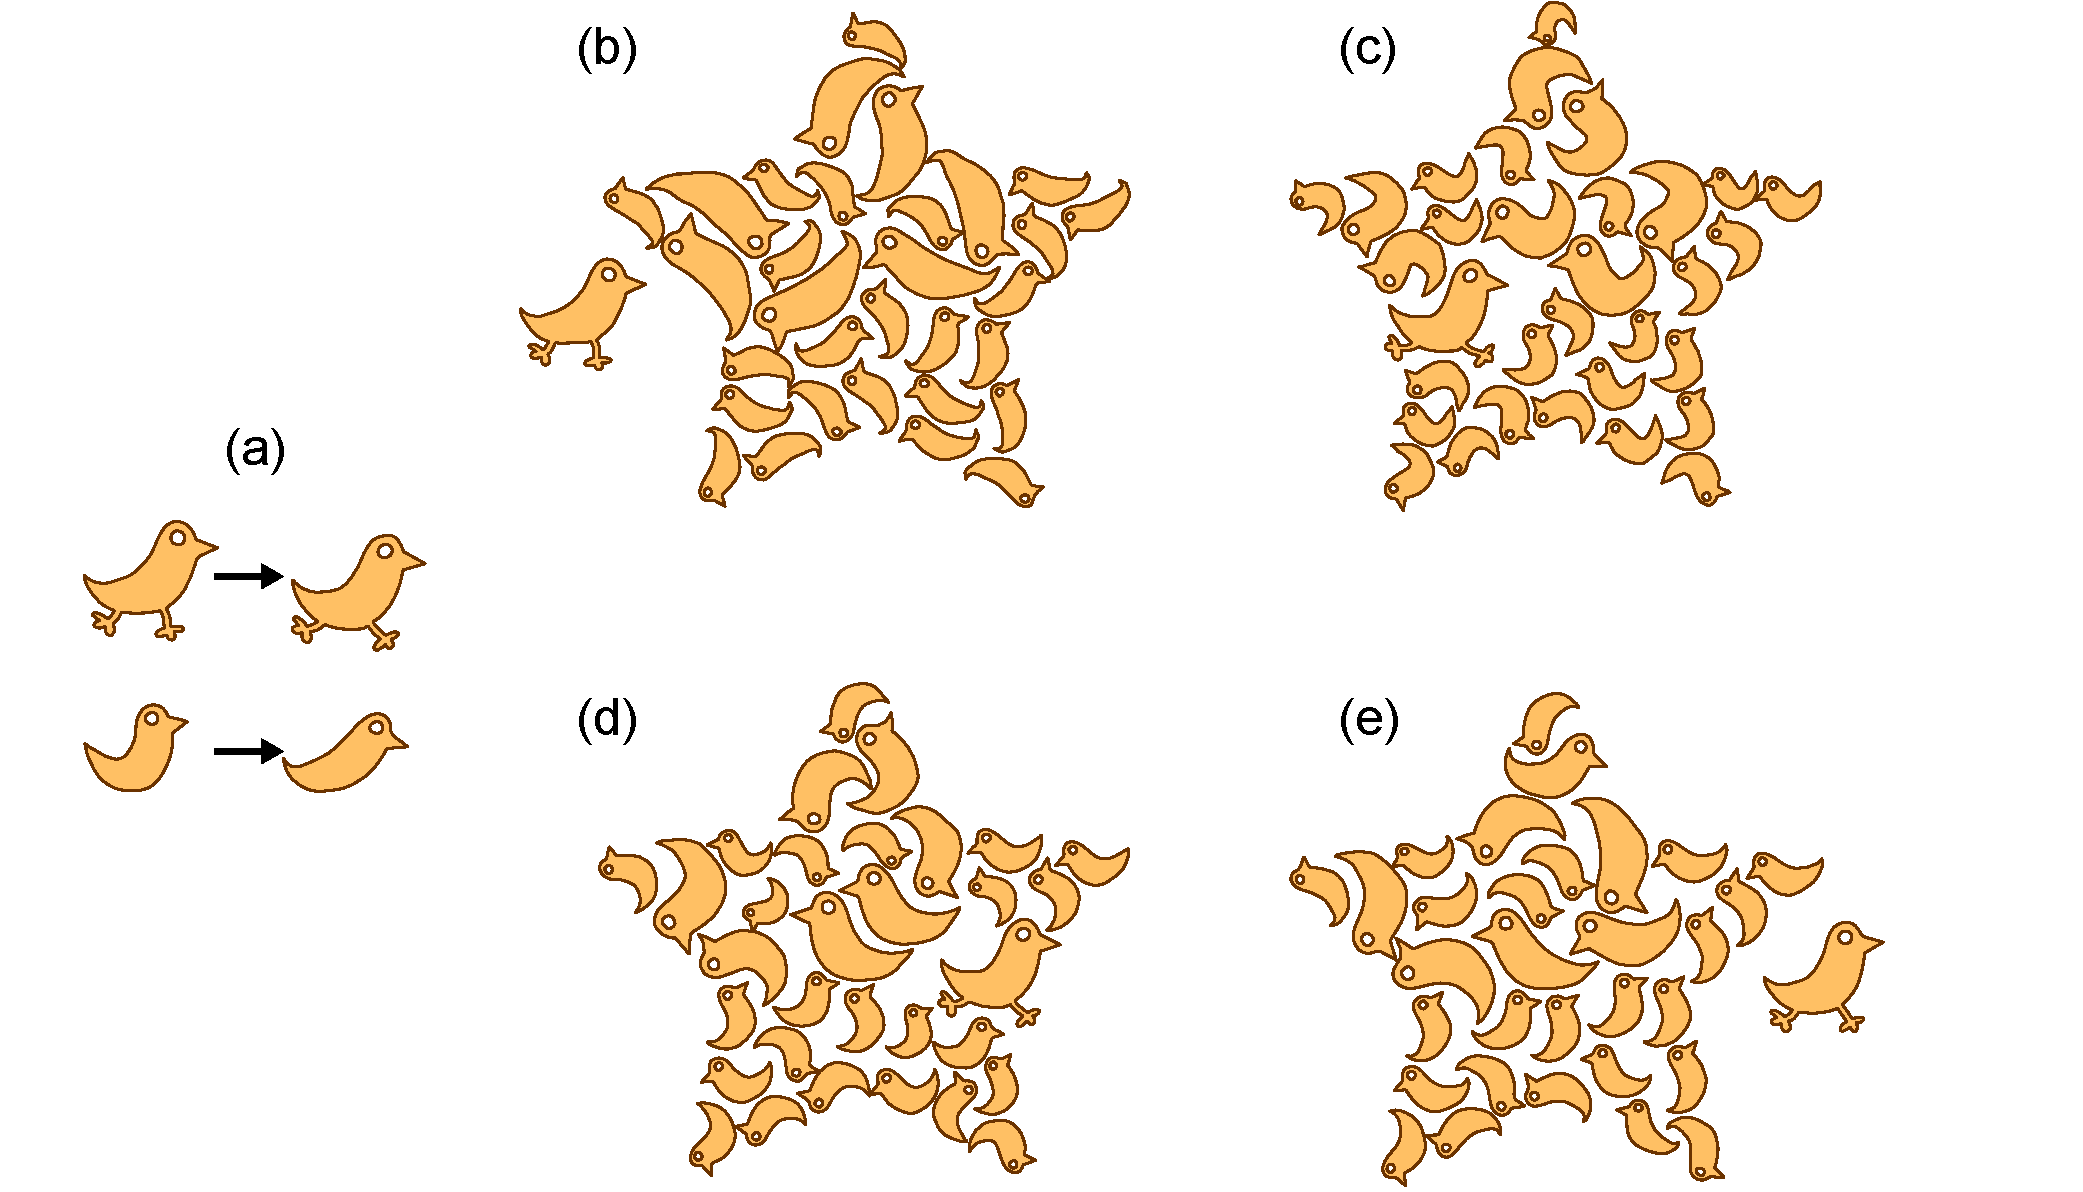
\includegraphics[width=1.0\textwidth]{figures/animationpak/birb_entering_star.pdf} 
\caption[An loose bird enters a packing of smaller birds inside a star]
{\label{fig_bib_entering_star} 
\newtext{An loose bird enters a star-shaped packing. 
The smaller birds shrink to give up their space to accommodate another element.}
}
\end{figure*}

\begin{figure*}
  \centering
  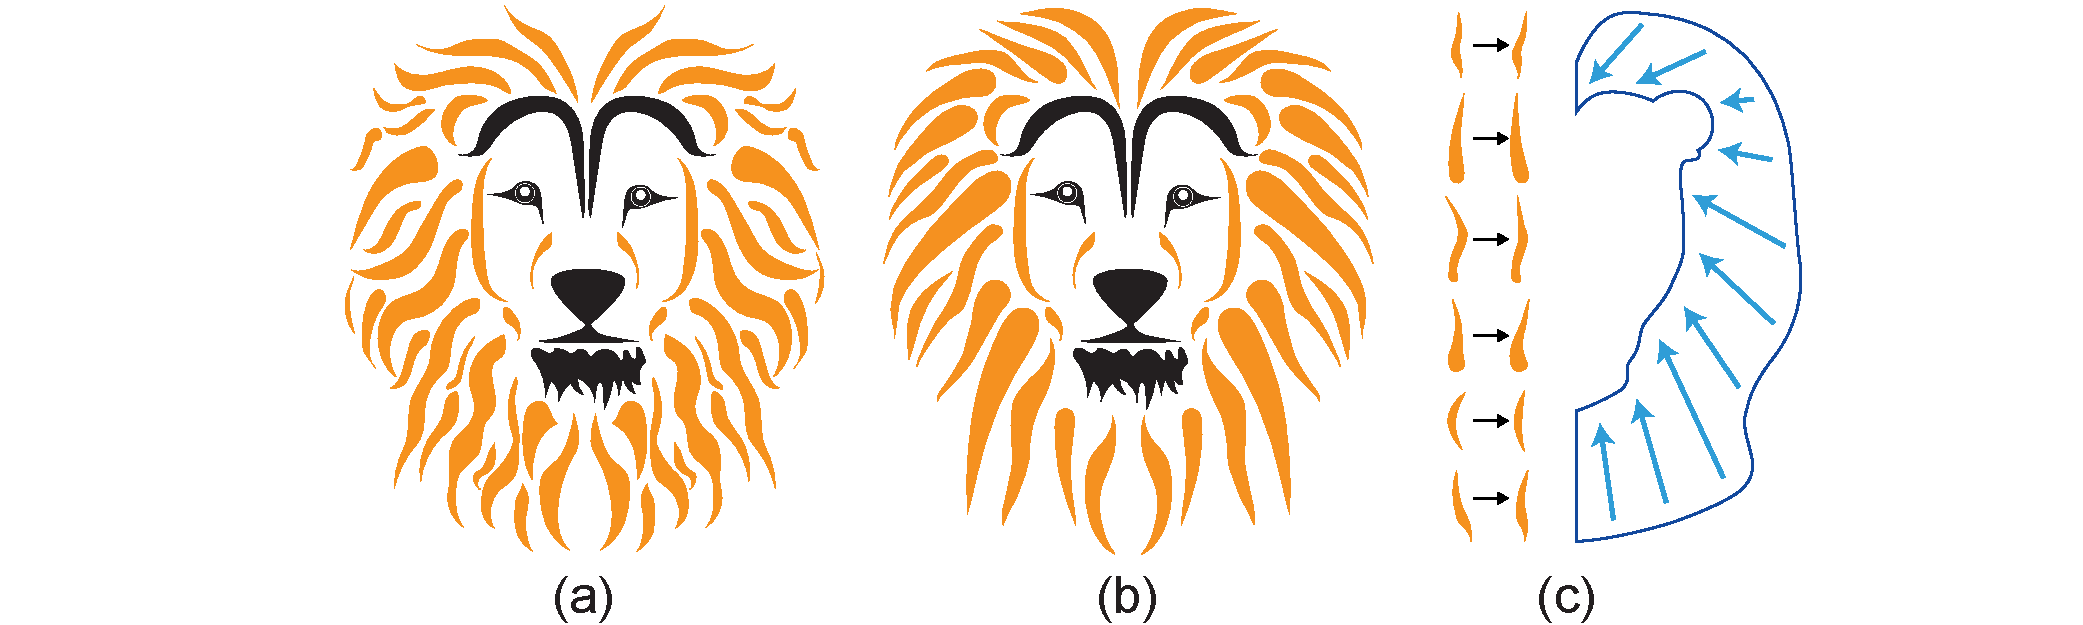
\includegraphics[width=1.0\textwidth]{figures/animationpak/lion_comparison.pdf}
  \caption[A packing of lion's mane]
  {
  \label{fig_animationpak_lion}
    (a) A static packing made by an artist, taken from StockUnlimited. 
  (b) The first frame from an AnimationPak packing. 
  (c) The input animated elements and the container shape with a vector field.
  Torsional forces keep elements oriented in the direction of the
  vector field.  We simulate half of the lion's mane and render the other
  half using a reflection, and add the facial features by hand.
  }  
\end{figure*}
\begin{figure*}
  \centering
  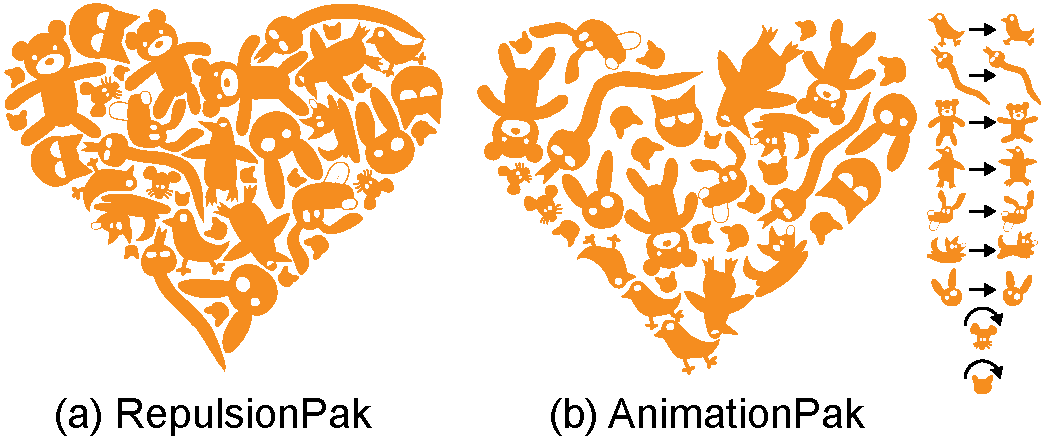
\includegraphics[width=1.0\textwidth]{figures/animationpak/repulsionpak_vs_animationpak.pdf}
  \caption[A comparison between RepulsionPak and AnimationPak]
  {
  \label{fig_animationpak_repulsionpak_vs_animationpak}
    (a) A static packing created with RepulsionPak.
  (b) The first frame of a comparable AnimationPak packing.
    The input spacetime elements are shown on the right.
  The AnimationPak packing has more negative space because
  we must tradeoff between temporal coherence and packing density.
  }  
\end{figure*}

\begin{figure*}
\centering
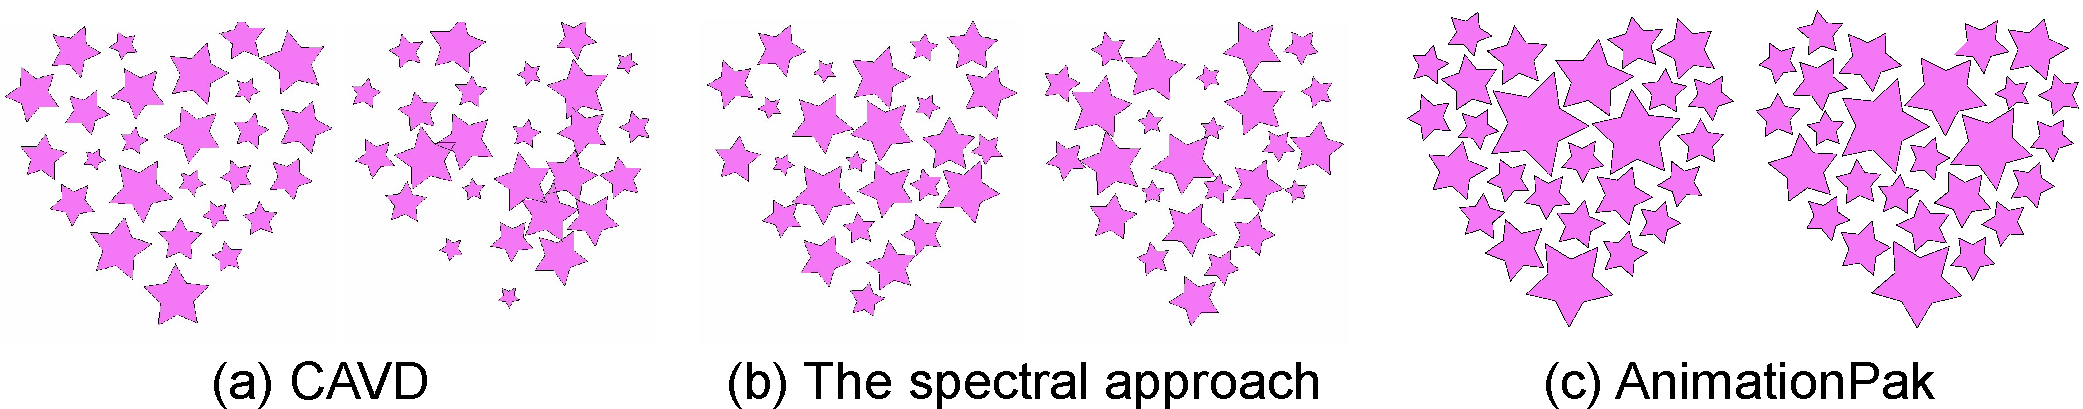
\includegraphics[width=1.0\textwidth]{figures/animationpak/star_comparison.pdf} 
\caption[An comparison between CAVD, The spectral approach, and AnimationPak]
{\label{fig_animationpak_star_comparison} 
A comparison of (a) Centroidal Area Voronoi Diagrams (CAVDs)~\cite{Smith2005}, 
(b) spectral packing~\cite{Dalal2006}, and (c) AnimationPak. 
We show two frames for each method, taken at $t = 0$ and $t = 0.5$. 
The CAVD packing starts with evenly distributed elements
but the packing degrades as the animation progresses.
The spectral approach improves upon CAVD with better consistency, 
but still leaves significant pockets of negative space.
The AnimationPak packing has less negative space that is more even.}
\end{figure*}





\begin{figure}[t]
\centering
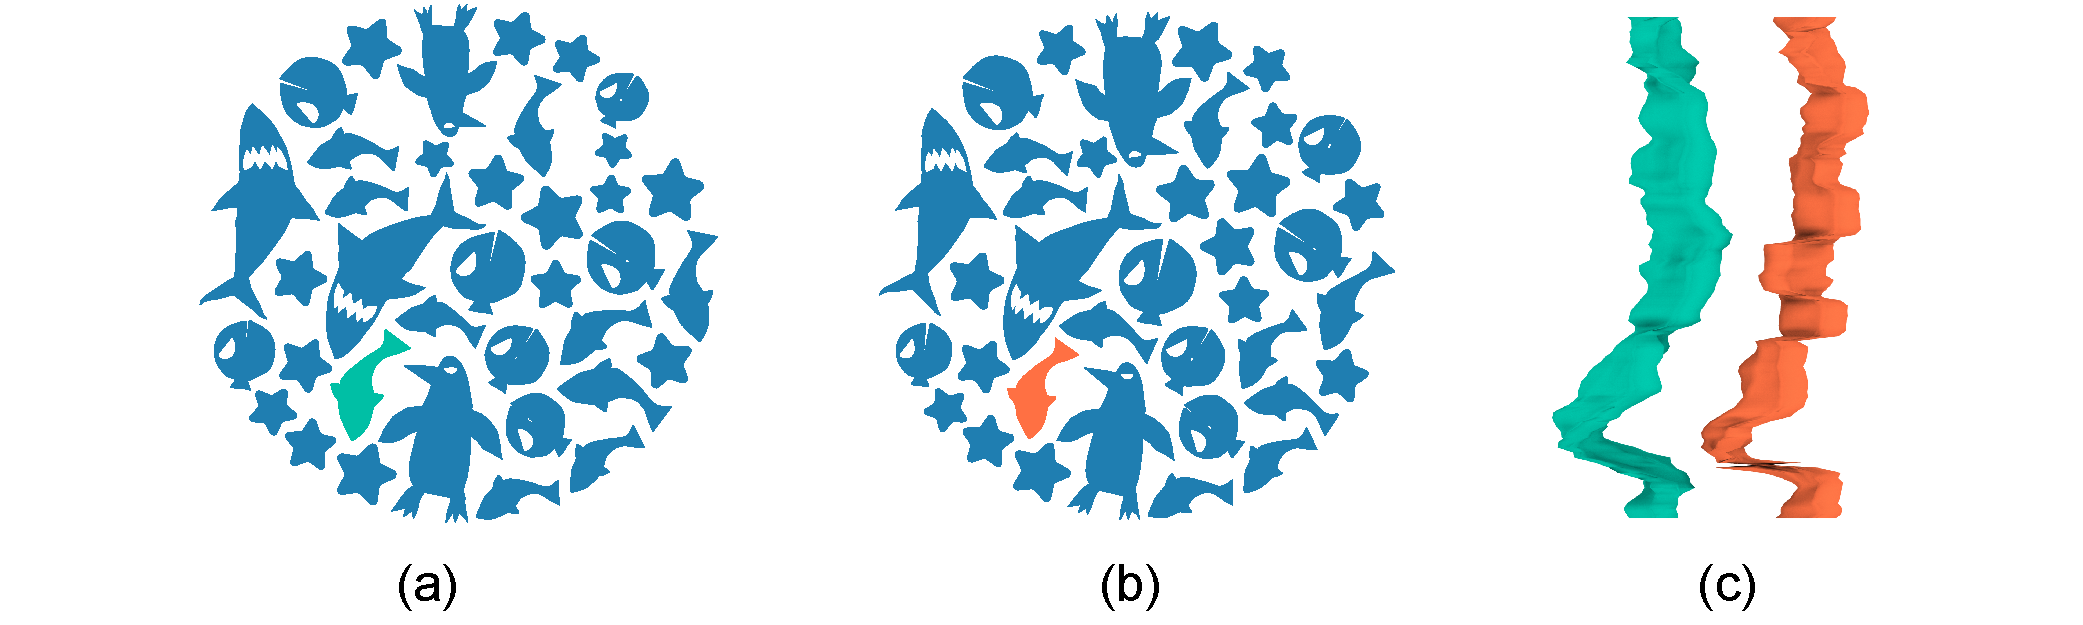
\includegraphics[width=1.0\textwidth]{figures/animationpak/teaser_weak_t_springs.pdf} 
\caption[The effect of adjusting time spring stiffness]
{\label{fig_animationpak_teaser_weak_t_springs} 
(a) One frame from Figure~\ref{fig_animationpak_teaser}.
(b) The same packing with time springs that are 1\% as stiff.
Reducing the stiffness of time springs leads to a more even packing with
less negative space, but the animated elements must move frantically to
preserve packing density.  
The spacetime trajectories of the highlighted
fish in (a) and (b) are shown in (c).  The orange fish in (b) exhibits more
high frequency fluctuation in its position.
}
\end{figure}

\begin{figure}[t]
\centering
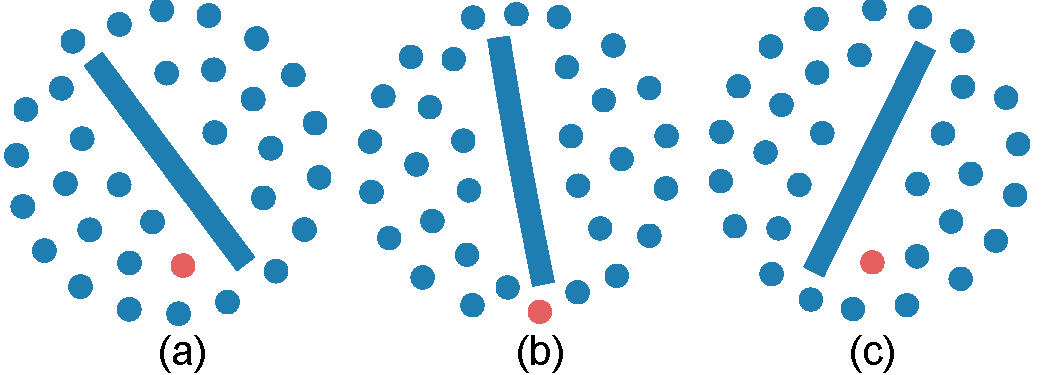
\includegraphics[width=1.0\textwidth]{figures/animationpak/blender.pdf} 
\caption[A failure case for AnimationPak]
{\label{fig_animationpak_blender} 
A failure case for AnimationPak, consisting of 
a rotating beam and a number of small circles.  Instead of being dragged
around by the beam, the circles dodge it entirely by sneaking through
the gap between the beam and the container.
The red circle demonstrates one such maneuver.
}
\end{figure}







